\documentclass[11pt,a4paper]{article}
\usepackage[utf8]{inputenc}
\usepackage[T1]{fontenc}
\usepackage[spanish,es-nodecimaldot,es-tabla]{babel}
\usepackage{lmodern,amsmath,amssymb,graphicx,pdfpages,booktabs,longtable,array,float,xcolor,listings,fancyhdr,titlesec,caption,needspace,microtype,xurl,hyperref}
\usepackage[top=2.3cm,bottom=2.3cm,left=2.2cm,right=2.2cm]{geometry}
\definecolor{azul}{HTML}{164769}
\definecolor{gris}{HTML}{F3F5F7}
\hypersetup{colorlinks=true,linkcolor=azul,urlcolor=azul,pdftitle={CVRP de logística urbana: etapa 2},pdfauthor={Equipo MA2015}}
\titleformat{\section}{\Large\bfseries}{\thesection.}{0.6em}{}
\titleformat{\subsection}{\large\bfseries}{\thesubsection.}{0.6em}{}
\titlespacing*{\section}{0pt}{16pt}{8pt}
\titlespacing*{\subsection}{0pt}{12pt}{6pt}
\setlength{\parindent}{0pt}\setlength{\parskip}{6pt}
\setlength{\emergencystretch}{2em}
\renewcommand{\arraystretch}{1.18}
\numberwithin{equation}{section}
\newcolumntype{P}[1]{>{\raggedright\arraybackslash}p{#1}}
\pagestyle{fancy}\fancyhf{}
\fancyhead[L]{\small Diseño de algoritmos matemáticos bioinspirados}
\fancyhead[R]{\small CVRP · Etapa 2}
\fancyfoot[C]{\thepage}\setlength{\headheight}{14pt}
\renewcommand{\headrulewidth}{0.3pt}
\captionsetup{font=small,labelfont=bf,justification=justified,singlelinecheck=false}
\lstset{basicstyle=\ttfamily\fontsize{8}{9.5}\selectfont,breaklines=true,columns=fullflexible,keepspaces=true,showstringspaces=false,frame=single,rulecolor=\color{black!18},backgroundcolor=\color{gris},xleftmargin=5pt,xrightmargin=5pt,framesep=5pt,tabsize=4,literate={á}{{\'a}}1 {é}{{\'e}}1 {í}{{\'i}}1 {ó}{{\'o}}1 {ú}{{\'u}}1 {ñ}{{\~n}}1 {ü}{{\"u}}1 {Ó}{{\'O}}1}
\begin{document}
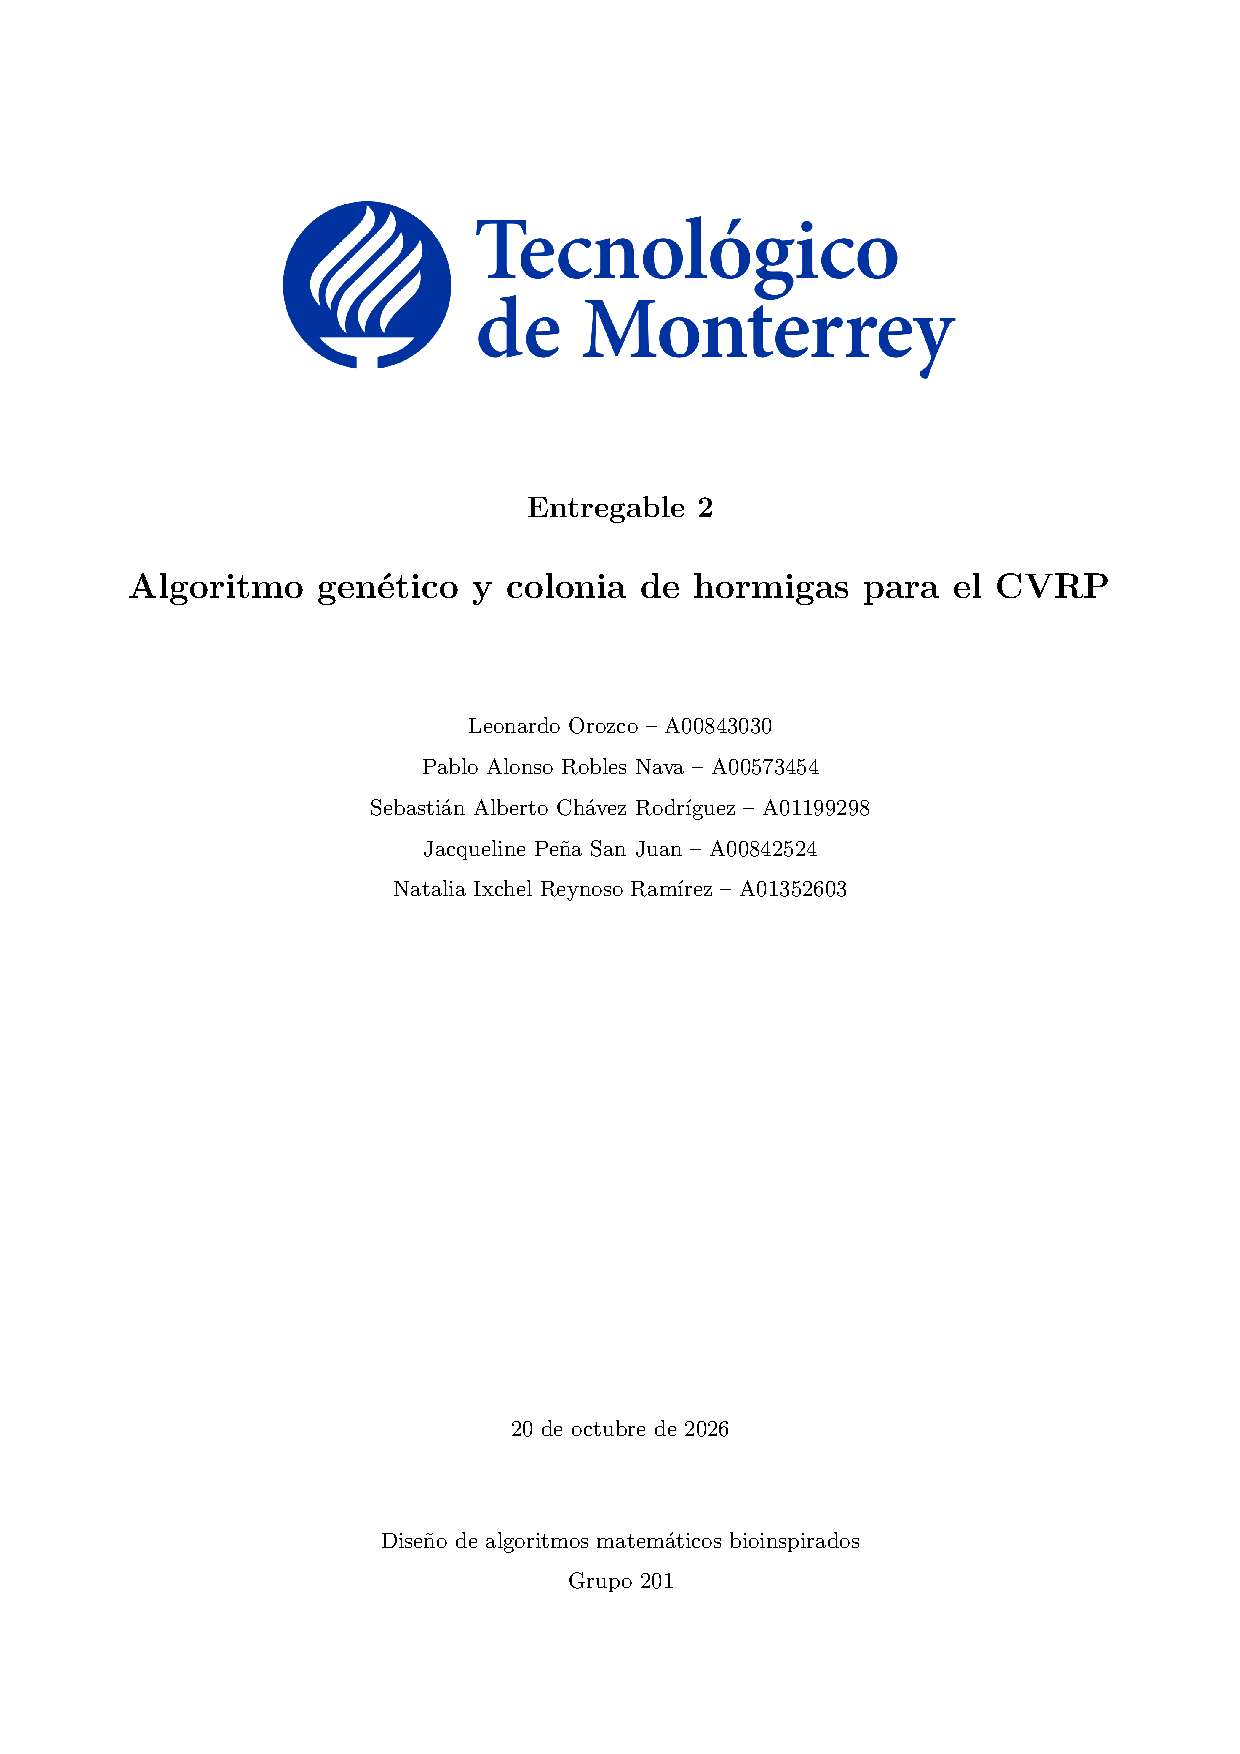
\includepdf[pages=1,fitpaper=true,pagecommand={\thispagestyle{empty}}]{portada_etapa2.pdf}
\setcounter{page}{2}

\section{Introducción y planteamiento experimental}

La etapa 1 estudió un problema de ruteo capacitado de diez clientes. La formulación exacta de arcos y flujo de producto obtuvo una distancia mínima de 318.989487 unidades; la heurística de ahorros de Clarke--Wright con 2-opt alcanzó 339.252870. Ambas soluciones emplearon cuatro rutas. La diferencia se debe a la asignación de clientes y al orden de visita: 2-opt mejora cada recorrido, pero conserva los clientes asignados a ese vehículo.

Esta etapa desarrolla dos métodos bioinspirados que modifican el orden global de los clientes: un algoritmo genético (GA) y un algoritmo de colonia de hormigas (ACO). Ambos utilizan el mismo decodificador Split, que transforma cada permutación en rutas factibles. El propósito es comparar calidad, uso de capacidad, variabilidad y tiempo frente a los dos métodos anteriores, manteniendo la misma instancia y convención de distancias.

Esta versión corregida conserva la configuración, las semillas y los resultados del experimento principal, que se reprodujeron exactamente. Añade ejemplos trabajados de Split, OX, inversión y construcción de una hormiga; el análisis de las dos corridas no óptimas del GA; la diversidad de ambas búsquedas; el efecto de la feromona sobre adyacencias que Split separa; una sensibilidad conjunta de los parámetros de ACO y del GA; y cinco instancias adicionales con óptimo certificado. El Anexo C relaciona cada observación de la revisión con la sección que la atiende.

\subsection{Instancia, objetivo y restricciones}

Se considera el grafo completo con nodos \(V=\{1,\dots,11\}\), depósito 1 y clientes \(C=\{2,\dots,11\}\). Cada ruta comienza y termina en el depósito; cada cliente se atiende una vez y sin dividir su demanda. La capacidad es \(Q=50\) y la demanda total, 146 unidades. La flota es homogénea y su tamaño no está prefijado. La Tabla~\ref{tab:datos} conserva los datos de la etapa 1.

\begin{table}[H]\centering\small
\caption{Datos de la instancia CVRP\_10.}\label{tab:datos}
\begin{tabular}{cccc}\toprule
Nodo & \(x\) & \(y\) & Demanda\\\midrule
1 & 50 & 50 & 0\\ 2 & 20 & 70 & 12\\ 3 & 30 & 80 & 18\\ 4 & 60 & 75 & 10\\ 5 & 80 & 70 & 15\\ 6 & 25 & 45 & 14\\
7 & 40 & 30 & 20\\ 8 & 65 & 25 & 16\\ 9 & 85 & 40 & 11\\ 10 & 45 & 60 & 13\\ 11 & 70 & 55 & 17\\\bottomrule
\end{tabular}
\end{table}

La distancia se calcula sin redondeo y se expresa en unidades geométricas:
\begin{equation}\label{eq:dist}
c_{ij}=\sqrt{(X_i-X_j)^2+(Y_i-Y_j)^2},\qquad c_{ii}=0.
\end{equation}
Se mantiene la variante euclidiana continua de la etapa 1, aunque el archivo didáctico lleve la etiqueta EUC\_2D. Para una colección de rutas \(R\), se minimiza
\begin{equation}\label{eq:obj}
Z(R)=\sum_{r\in R}\ \sum_{(i,j)\ \text{consecutivos en } r} c_{ij},\qquad L_r=\sum_{i\ \text{atendido en } r} q_i\le Q .
\end{equation}
La cantidad de rutas satisface \(m\ge\lceil 146/50\rceil=3\). Esta cota no obliga a elegir tres: la solución de mínima distancia usa cuatro. El óptimo de tres rutas, 339.164674, se conserva como referencia de la etapa 1, pero no es el objetivo impuesto a GA o ACO.

\Needspace{12\baselineskip}
\subsection{Decodificación común mediante Split}

Una permutación \(\pi=(\pi_1,\dots,\pi_{10})\) contiene cada cliente exactamente una vez. Se divide en segmentos consecutivos; cada segmento origina una ruta desde y hacia el depósito. Para \(1\le a\le b\le 10\), su carga y su costo son
\begin{equation}\label{eq:seg}
L_{ab}=\sum_{k=a}^{b} q_{\pi_k},\qquad w_{ab}=c_{1,\pi_a}+\sum_{k=a}^{b-1} c_{\pi_k,\pi_{k+1}}+c_{\pi_b,1}.
\end{equation}
El costo mínimo del prefijo de longitud \(b\) se obtiene por programación dinámica. La minimización considera únicamente segmentos cuya carga satisface \(L_{ab}\le Q\):
\begin{equation}\label{eq:split}
D(0)=0,\qquad D(b)=\min_{\substack{1\le a\le b\\ L_{ab}\le Q}}\{D(a-1)+w_{ab}\},\qquad \mathrm{pred}(b)=a^*-1 .
\end{equation}
\(a^*\) es el índice que alcanza el mínimo. \(D(10)\) es la evaluación de la permutación y los predecesores reconstruyen las rutas, como se muestra en la sección~\ref{sec:ejsplit}. La idea de separar una secuencia sin delimitadores mediante Split se apoya en Prins (2004). Aquí se implementa una versión cuadrática y sin búsqueda local adicional. Split encuentra la mejor división \emph{para el orden dado}; la búsqueda global de ese orden corresponde a GA o ACO.

El decodificador puede cerrar una ruta aun cuando quede capacidad disponible. Esto permite representar la ruta individual del cliente 10 presente en el óptimo. Todo cliente tiene demanda menor que 50, de modo que cualquier permutación admite al menos la partición en rutas individuales. No se requieren penalizaciones por sobrecarga ni reparación de soluciones.

\Needspace{14\baselineskip}
\subsection{Ejemplo de Split: cortes, cargas, costos y predecesores}\label{sec:ejsplit}

Se toma como ejemplo el mejor cromosoma de la semilla 0 del GA, \(\pi=(4,5,11,6,2,3,10,7,8,9)\), cuyas demandas en ese orden son \((10,15,17,14,12,18,13,20,16,11)\). La Tabla~\ref{tab:splitdp} muestra cada etiqueta \(D(b)\), su predecesor y el segmento que la produce. Para \(b=7\), la Tabla~\ref{tab:splitb7} lista los candidatos: los segmentos que empiezan en \(a\le 4\) superan la capacidad y no se evalúan, y el mínimo se obtiene cerrando una ruta sólo con el cliente 10.

\begin{table}[H]\centering\small
\caption{Etiquetas de Split para \(\pi=(4,5,11,6,2,3,10,7,8,9)\). La columna \(w_{ab}\) es el costo de la última ruta, definida por \(a=\mathrm{pred}(b)+1\).}\label{tab:splitdp}
\begin{tabular}{rrrrrlrr}\toprule
$b$ & $\pi_b$ & $q_{\pi_b}$ & $D(b)$ & $\mathrm{pred}(b)$ & Último segmento que da $D(b)$ & Carga & $w_{ab}$\\\midrule
1 & 4 & 10 & 53.851648 & 0 & $(\pi_{1},\dots,\pi_{1})=(4)$ & 10 & 53.851648\\
2 & 5 & 15 & 83.596865 & 0 & $(\pi_{1},\dots,\pi_{2})=(4, 5)$ & 25 & 83.596865\\
3 & 11 & 17 & 86.184637 & 0 & $(\pi_{1},\dots,\pi_{3})=(4, 5, 11)$ & 42 & 86.184637\\
4 & 6 & 14 & 137.174832 & 3 & $(\pi_{4},\dots,\pi_{4})=(6)$ & 14 & 50.990195\\
5 & 2 & 12 & 173.230345 & 3 & $(\pi_{4},\dots,\pi_{5})=(6, 2)$ & 26 & 87.045708\\
6 & 3 & 18 & 187.372480 & 3 & $(\pi_{4},\dots,\pi_{6})=(6, 2, 3)$ & 44 & 101.187844\\
7 & 10 & 13 & 209.733160 & 6 & $(\pi_{7},\dots,\pi_{7})=(10)$ & 13 & 22.360680\\
8 & 7 & 20 & 251.327312 & 6 & $(\pi_{7},\dots,\pi_{8})=(10, 7)$ & 33 & 63.954832\\
9 & 8 & 16 & 283.616490 & 6 & $(\pi_{7},\dots,\pi_{9})=(10, 7, 8)$ & 49 & 96.244010\\
10 & 9 & 11 & 318.989487 & 7 & $(\pi_{8},\dots,\pi_{10})=(7, 8, 9)$ & 47 & 109.256327\\
\bottomrule\end{tabular}

\end{table}

\begin{table}[H]\centering\small
\caption{Candidatos evaluados para la etiqueta \(D(7)\).}\label{tab:splitb7}
\begin{tabular}{rrlr}\toprule
$a$ & $L_{a7}$ & Candidato & Valor\\\midrule
4 & 57 & \multicolumn{2}{l}{excede $Q=50$: no se evalúa}\\
5 & 43 & $D(4)+w_{5,7}=137.174832+86.377988$ & 223.552820\\
6 & 31 & $D(5)+w_{6,7}=173.230345+72.235853$ & 245.466197\\
7 & 13 & $D(6)+w_{7,7}=187.372480+22.360680$ & 209.733160 $\leftarrow$ mínimo\\
\bottomrule\end{tabular}

\end{table}

La reconstrucción parte de \(b=10\) y sigue los predecesores hacia atrás:
\[
\mathrm{pred}(10)=7\Rightarrow(7,8,9),\quad
\mathrm{pred}(7)=6\Rightarrow(10),\quad
\mathrm{pred}(6)=3\Rightarrow(6,2,3),\quad
\mathrm{pred}(3)=0\Rightarrow(4,5,11).
\]
Los cortes quedan después de las posiciones 3, 6 y 7. Las rutas, en el orden del cromosoma, son \(1\to4\to5\to11\to1\) (carga 42), \(1\to6\to2\to3\to1\) (44), \(1\to10\to1\) (13) y \(1\to7\to8\to9\to1\) (47), con \(D(10)=318.989487=Z^*\). Un corte voraz que llenara cada vehículo hasta que el siguiente cliente no cupiera produciría \((4,5,11)\,|\,(6,2,3)\,|\,(10,7,8)\,|\,(9)\), con 356.417589 unidades. La diferencia de 37.428 unidades muestra por qué Split evalúa todos los cortes factibles en lugar de llenar los vehículos. Las \(2^9=512\) formas de cortar esta permutación se comparan automáticamente con Split en la prueba \texttt{test\_split\_caso\_fijo\_del\_informe} (sección~\ref{sec:protocolo}).

\section{Algoritmo genético}

\subsection{Representación, aptitud y operadores}

El cromosoma es una permutación de los diez clientes. Su evaluación es \(Z(\pi)=D(10)\), que se minimiza directamente. Un torneo binario selecciona dos individuos diferentes y elige el de menor costo; dos torneos independientes eligen los padres. La inicialización genera permutaciones aleatorias, sin incluir previamente la solución exacta ni la de Clarke--Wright.

La cruza OX conserva un segmento del primer padre y completa las posiciones restantes en el orden circular del segundo, evitando duplicaciones. La mutación invierte un segmento elegido al azar. Ambos operadores preservan la cobertura de los diez clientes y pueden cambiar la agrupación de las rutas después de Split. El reemplazo conserva los dos mejores padres y los 18 mejores hijos. Se admiten cromosomas repetidos; la sección~\ref{sec:diversidad} mide el efecto de esta elección sobre la diversidad.

\Needspace{12\baselineskip}
\subsection{Ejemplo de OX y de inversión de segmento}\label{sec:ejox}

Se usan los dos primeros individuos de la población inicial de la semilla 0 y un segmento fijo, las posiciones 4 a 7, para que el cálculo pueda seguirse a mano (Tabla~\ref{tab:ox}).

\begin{table}[H]\centering\small
\caption{Cruza OX entre \(a\) y \(b\) con segmento en las posiciones 4--7, seguida de la inversión de las posiciones 2--5. En negritas, los genes copiados o invertidos.}\label{tab:ox}
\begin{tabular}{l*{10}{c}}\toprule
Posición & 1 & 2 & 3 & 4 & 5 & 6 & 7 & 8 & 9 & 10\\\midrule
Padre $a$ & 8 & 11 & 2 & \textbf{4} & \textbf{6} & \textbf{5} & \textbf{7} & 3 & 10 & 9\\
Padre $b$ & 11 & 5 & 4 & 9 & 3 & 2 & 8 & 10 & 6 & 7\\
Orden circular de $b$ desde la posición 8 & \multicolumn{10}{l}{10, 6, 7, 11, 5, 4, 9, 3, 2, 8}\\
Sin los genes ya copiados & \multicolumn{10}{l}{10, 11, 9, 3, 2, 8}\\
Hijo OX & 3 & 2 & 8 & \textbf{4} & \textbf{6} & \textbf{5} & \textbf{7} & 10 & 11 & 9\\
Hijo invertido ($i=2$, $j=5$) & 3 & \textbf{6} & \textbf{4} & \textbf{8} & \textbf{2} & 5 & 7 & 10 & 11 & 9\\
\bottomrule\end{tabular}

\end{table}

\begin{enumerate}
\item El hijo copia de \(a\) el segmento de las posiciones 4--7: \((4,6,5,7)\).
\item Se recorre \(b\) circularmente desde la posición 8: \(10,6,7,11,5,4,9,3,2,8\).
\item Se descartan los clientes ya copiados (4, 5, 6 y 7) y queda \(10,11,9,3,2,8\).
\item Esos clientes llenan, en orden, las posiciones 8, 9, 10, 1, 2 y 3. El hijo es \((3,2,8,4,6,5,7,10,11,9)\).
\end{enumerate}

\textbf{Verificación:} el hijo contiene \(\{2,3,\dots,11\}\) y cada cliente aparece una sola vez. Split lo divide en \((3,2)\,|\,(8,4,6)\,|\,(5,7)\,|\,(10,11,9)\), con \(Z=446.524044\); el hijo mejora al padre \(a\) (485.305878) pero no al \(b\) (378.853929). La inversión de las posiciones 2--5 da \((3,6,4,8,2,5,7,10,11,9)\), que tampoco repite ni omite clientes; Split lo divide en \((3,6,4)\,|\,(8)\,|\,(2,5,7)\,|\,(10,11,9)\) y vale 472.017842. Ambos operadores sólo cambian el orden, por lo que no pueden producir infactibilidad. Como muestra el ejemplo, pueden mejorar o empeorar el costo: su función es explorar, y la selección decide qué cambios se conservan. La prueba \texttt{test\_ox\_e\_inversion\_conservan\_permutacion} repite esta comprobación en 1,000 cruces e inversiones.

\Needspace{14\baselineskip}
\subsection{Hiperparámetros y justificación}

\begin{table}[H]\centering\small
\caption{Configuración principal del algoritmo genético.}\label{tab:gaparam}
\begin{tabular}{p{4.2cm}p{3cm}p{7.4cm}}\toprule
Parámetro & Valor & Justificación\\\midrule
Población & 20 & Dos veces el número de clientes; mantiene alternativas con bajo costo.\\
Etapas & 100 & Inicialización y 99 generaciones de descendencia; presupuesto fijo.\\
Cruza \(p_c\) & 0.90 & Favorece recombinar el orden de clientes.\\
Mutación \(p_m\) & 0.20 por hijo & Introduce inversiones sin alterar todos los descendientes.\\
Torneo & 2 & Presión selectiva moderada y fácil de reproducir.\\
Elitismo & 2 individuos & Retiene el mejor costo y una segunda alternativa.\\
Semillas & 0--9 & Diez corridas para observar variación estocástica.\\
Búsqueda local & Ninguna & Permite evaluar la combinación de evolución y Split.\\\bottomrule
\end{tabular}
\end{table}

Estos valores se fijaron antes de observar las diez corridas principales y no se presentan como una calibración óptima; la sección~\ref{sec:sens} evalúa sus alternativas.

\textbf{Conteo de evaluaciones.} Cada corrida evalúa \(20+99\times20=2000\) cromosomas: los 20 de la población inicial y 1,980 hijos. Una evaluación es una llamada a Split que devuelve \(Z(\pi)\). Al terminar, el programa decodifica una vez más el mejor cromosoma para obtener sus rutas; esa llamada no se cuenta en las 2,000 evaluaciones, pero sí está dentro del tiempo medido. Por esta razón, el número de evaluaciones mide el esfuerzo de búsqueda y no el tiempo: el tiempo incluye además la selección, la cruza, la mutación y el reemplazo (sección~\ref{sec:tiempos}). El número de permutaciones posibles es \(10!=3\,628\,800\), por lo que el presupuesto no representa una enumeración exhaustiva.

\subsection{Programación y pseudocódigo}

La función \texttt{ga} controla población y generaciones; \texttt{ox} implementa la cruza y \texttt{split} calcula aptitud y rutas. La semilla alimenta una instancia local de \texttt{random.Random}, independiente de otras ejecuciones. El Anexo A contiene la implementación completa de los dos métodos y del decodificador.

\Needspace{14\baselineskip}
\begin{lstlisting}[caption={Pseudocódigo del algoritmo genético.}]
Crear 20 permutaciones aleatorias; evaluar cada una con Split   (evaluaciones 1-20)
Registrar el mejor costo inicial
Repetir 99 generaciones:
    Para cada uno de 20 hijos:
        Elegir dos padres mediante torneos binarios independientes
        Aplicar OX con probabilidad 0.90; de otro modo copiar al primero
        Invertir un segmento con probabilidad 0.20
        Evaluar el hijo mediante Split                          (20 evaluaciones por generacion)
    Conservar los 2 mejores padres y los 18 mejores hijos
    Registrar el mejor costo acumulado
Decodificar el mejor cromosoma (no se cuenta como evaluacion) y devolver costo, rutas e historial
\end{lstlisting}

\Needspace{12\baselineskip}
\subsection{Validación y rutas obtenidas}

El GA alcanzó \(Z^*=318.989487\) en ocho de las diez semillas principales. Su media fue 321.958694 y su peor resultado, 336.713769. Para mostrar la solución se elige la semilla 0, que alcanzó el óptimo, y se ordenan las rutas sólo para facilitar la lectura. Invertir un recorrido no cambia su costo porque las distancias son simétricas.

\begin{table}[H]\centering\small
\caption{Rutas de GA + Split, semilla 0.}\label{tab:rutasga}
\begin{tabular}{llrrr}\toprule
Ruta & Recorrido & Distancia & Carga / 50 & Libre (\%)\\\midrule
R1 & \(1\to10\to1\) & 22.360680 & 13 & 74\\
R2 & \(1\to3\to2\to6\to1\) & 101.187844 & 44 & 12\\
R3 & \(1\to4\to5\to11\to1\) & 86.184637 & 42 & 16\\
R4 & \(1\to7\to8\to9\to1\) & 109.256327 & 47 & 6\\\bottomrule
\end{tabular}
\end{table}

La capacidad no utilizada por ruta y la utilización global se calculan como
\begin{equation}\label{eq:util}
U_r=100\,\frac{Q-L_r}{Q},\qquad \text{Utilización}=100\,\frac{146}{mQ}.
\end{equation}
Las cuatro rutas transportan 146 unidades de 200 disponibles: utilización de 73\% y espacio libre global de 27\%. La ruta del cliente 10 deja 74\% libre, pero reduce la distancia total al permitir una mejor distribución de los otros clientes.

\begin{figure}[H]\centering
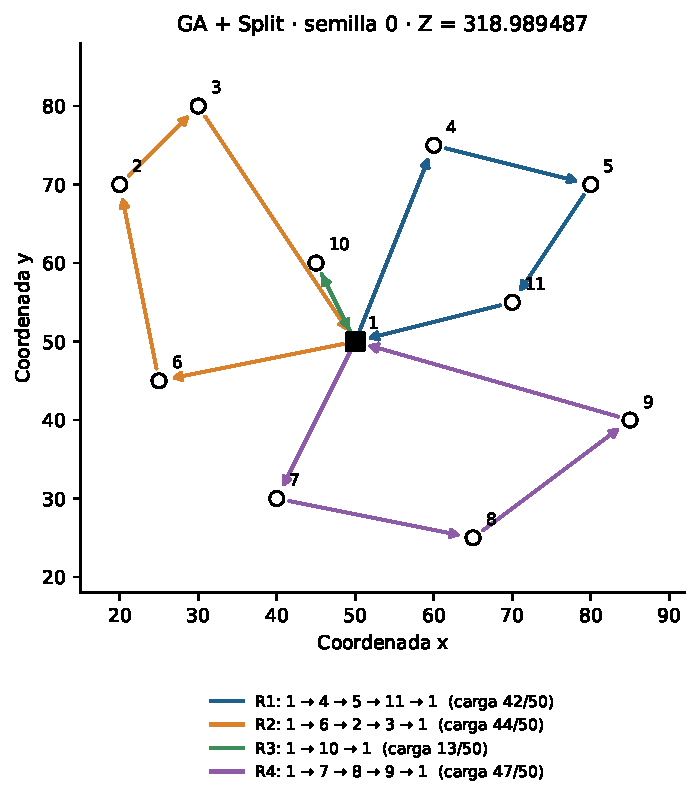
\includegraphics[width=.62\linewidth]{figuras/fig1_rutas_ga.pdf}
\caption{Mejor solución del algoritmo genético (semilla 0). Las flechas indican el sentido y el cuadrado, el depósito.}\label{fig:rutasga}
\end{figure}

La Figura~\ref{fig:rutasga} distingue tres grupos geográficos y la ruta corta al cliente 10. A diferencia de la solución de Clarke--Wright de la etapa 1, el cliente 11 se integra con 4 y 5, y el 9 con 7 y 8. Esta reasignación explica que el algoritmo pueda superar una mejora limitada al interior de cada ruta.

\textbf{Soluciones no óptimas.} La Tabla~\ref{tab:rutas48} y la Figura~\ref{fig:rutas48} muestran las soluciones finales de las semillas 4 y 8, que también se verificaron: cada cliente aparece una vez, todas las rutas salen y regresan al depósito, ninguna carga supera 50 y la suma de arcos coincide con el valor reportado. Ambas usan cuatro rutas y 73\% de la capacidad, igual que el óptimo, así que su GAP no proviene de la capacidad sino de la agrupación. En la semilla 4, el cliente 7 queda solo, el 10 se une con 4 y 5 y el 11 con 9 y 8; el óptimo une 7 con 8 y 9, el 11 con 4 y 5 y deja solo al 10. En la semilla 8, el 4 se agrupa con 3 y 2, el 6 con 7 y 8, y el 9 con 11 y 5; sólo la ruta individual del cliente 10 coincide con el óptimo.

\begin{table}[H]\centering\small
\caption{Rutas finales de las semillas no óptimas del GA.}\label{tab:rutas48}
\begin{tabular}{rllrrr}\toprule
Semilla & Ruta & Recorrido & Distancia & Carga / 50 & Libre (\%)\\\midrule
4 & R1 & 1$\to$11$\to$9$\to$8$\to$1 & 95.983491 & 44 & 12\\
4 & R2 & 1$\to$3$\to$2$\to$6$\to$1 & 101.187844 & 44 & 12\\
4 & R3 & 1$\to$7$\to$1 & 44.721360 & 20 & 60\\
4 & R4 & 1$\to$10$\to$4$\to$5$\to$1 & 89.064584 & 38 & 24\\
\addlinespace
8 & R1 & 1$\to$11$\to$5$\to$9$\to$1 & 105.457647 & 43 & 14\\
8 & R2 & 1$\to$10$\to$1 & 22.360680 & 13 & 74\\
8 & R3 & 1$\to$6$\to$7$\to$8$\to$1 & 101.358158 & 50 & 0\\
8 & R4 & 1$\to$4$\to$3$\to$2$\to$1 & 107.537285 & 40 & 20\\
\bottomrule\end{tabular}

\end{table}

\begin{figure}[H]\centering
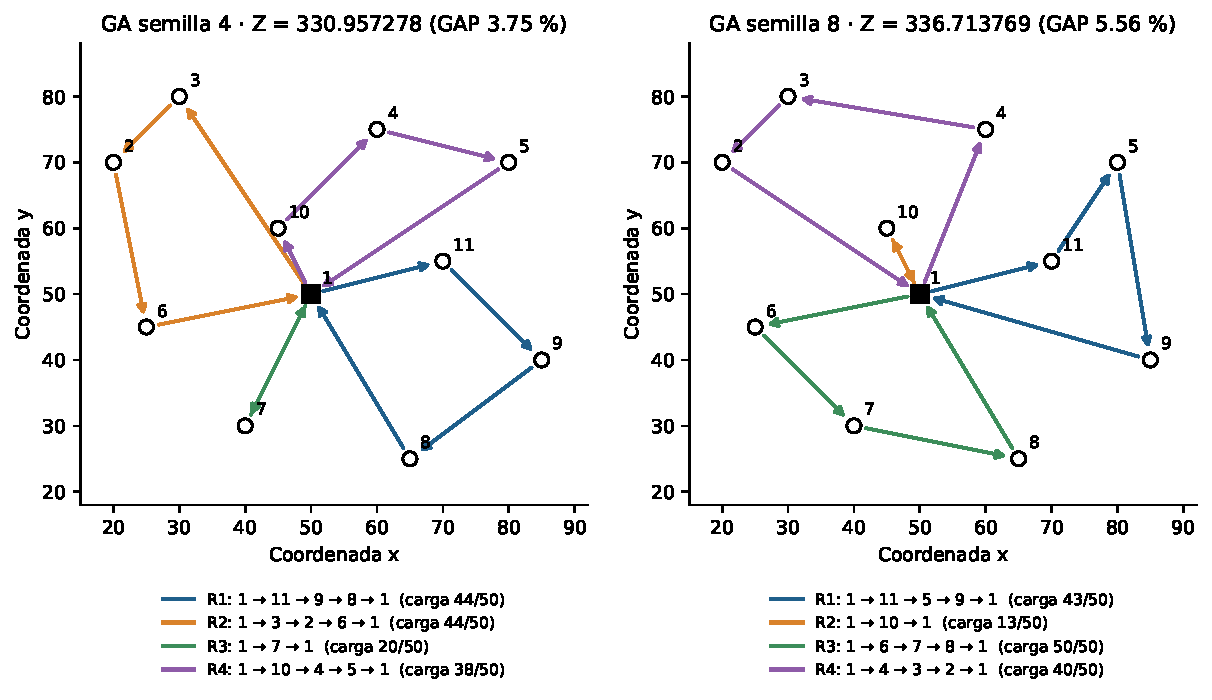
\includegraphics[width=\linewidth]{figuras/fig_rutas_semillas_4_8.pdf}
\caption{Soluciones finales de las semillas 4 y 8 del GA.}\label{fig:rutas48}
\end{figure}

\Needspace{14\baselineskip}
\subsection{Diversidad y causas de las corridas no óptimas}\label{sec:diversidad}

Para estudiar la diversidad se repitieron las diez corridas con una copia instrumentada del GA que hace las mismas llamadas al generador aleatorio; los diez valores finales coinciden con la Tabla~\ref{tab:individual}. En cada generación se registran tres medidas de la población: cromosomas distintos, soluciones distintas después de Split (dos permutaciones pueden producir las mismas rutas) y la distancia media de adyacencias. Esta última vale \(1-|A\cap B|/11\) para cada par de permutaciones, donde \(A\) y \(B\) son las 11 aristas del ciclo depósito--permutación--depósito; es 0 si dos individuos describen el mismo ciclo y 1 si no comparten aristas.

\begin{figure}[H]\centering
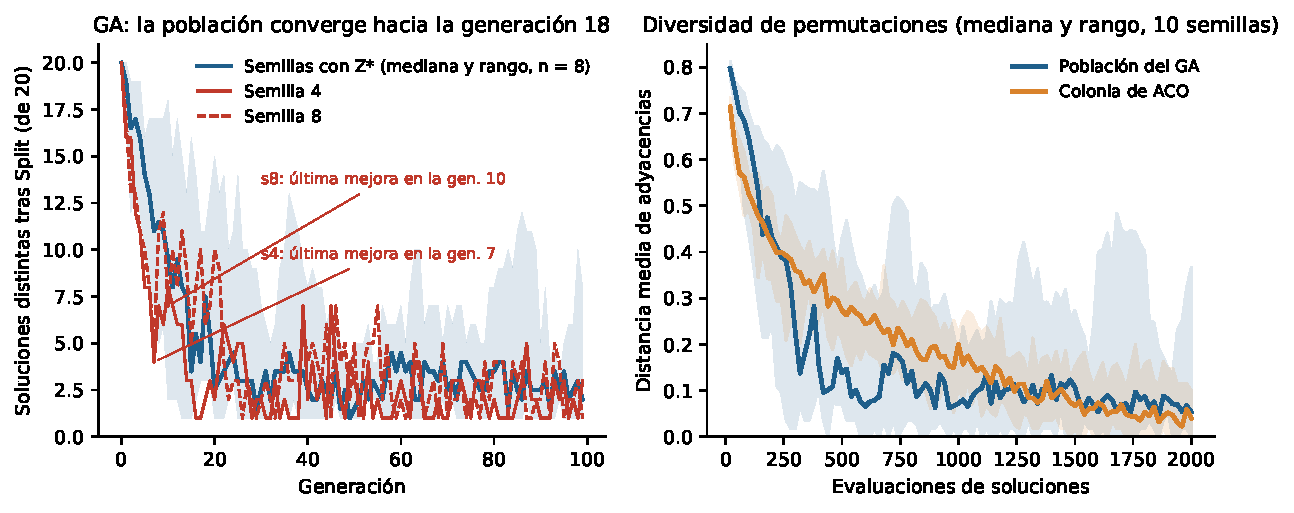
\includegraphics[width=\linewidth]{figuras/fig_diversidad.pdf}
\caption{Izquierda: soluciones distintas después de Split en la población del GA. Derecha: diversidad de permutaciones del GA y de la colonia de ACO por evaluación (mediana y rango de las semillas 0--9).}\label{fig:diversidad}
\end{figure}

La diversidad cae rápido en todas las semillas (Figura~\ref{fig:diversidad}). La población inicial tiene 20 soluciones distintas y una distancia de adyacencias de 0.78. Hacia la generación 18, la población queda reducida por primera vez a tres o menos soluciones distintas, tanto en las semillas exitosas (generación 17.1 en promedio) como en las fallidas (18.5). Entre las generaciones 10 y 99, las semillas que llegan al óptimo promedian 3.9 soluciones distintas y una distancia de 0.147; las semillas 4 y 8, 3.1 y 0.105. La diferencia es pequeña: la pérdida de diversidad afecta a todas las corridas y, por sí sola, no distingue las fallidas.

Lo que distingue a las fallidas es dónde ocurre esa convergencia. La Tabla~\ref{tab:mejoras48} muestra la evolución del mejor cromosoma. La semilla 4 deja de mejorar en la evaluación 154 (generación 7) y la semilla 8 en la 212 (generación 10), es decir, antes de que la población pierda su diversidad. A partir de ahí, la población queda formada por variantes de un mismo cromosoma.

\begin{table}[H]\centering\small
\caption{Evolución del mejor cromosoma en las semillas 4 y 8. Cada fila es una mejora; las barras separan las rutas que define Split.}\label{tab:mejoras48}
\begin{tabular}{rrrrrl}\toprule
Semilla & Generación & Evaluación & Mejor $Z$ & GAP (\%) & Rutas después de Split (clientes)\\\midrule
4 & 0 & 20 & 365.921866 & 14.71 & 5,4 $|$ 7,10 $|$ 9,11,8 $|$ 3,2,6\\
4 & 1 & 30 & 351.315978 & 10.13 & 5,9,8 $|$ 3,2 $|$ 7,6 $|$ 10,4,11\\
4 & 2 & 46 & 345.492246 & 8.31 & 5,4,10 $|$ 9,11 $|$ 3,2,6 $|$ 8,7\\
4 & 4 & 82 & 339.252870 & 6.35 & 10,4,5,9 $|$ 11 $|$ 3,2,6 $|$ 8,7\\
4 & 7 & 154 & 330.957278 & 3.75 & 11,9,8 $|$ 3,2,6 $|$ 7 $|$ 10,4,5\\
\addlinespace
8 & 0 & 11 & 372.840765 & 16.88 & 4 $|$ 6,3,2 $|$ 5,11,9 $|$ 10,7,8\\
8 & 2 & 54 & 366.737801 & 14.97 & 6,3,2 $|$ 5,9,11 $|$ 10 $|$ 7,8,4\\
8 & 4 & 95 & 366.468512 & 14.88 & 6 $|$ 4,3,2 $|$ 5,11,9 $|$ 10,7,8\\
8 & 5 & 101 & 359.075011 & 12.57 & 6,3,2 $|$ 5,11,9 $|$ 4,10 $|$ 7,8\\
8 & 7 & 143 & 353.427846 & 10.80 & 4,3,2 $|$ 9,5,11 $|$ 10 $|$ 7,8,6\\
8 & 9 & 185 & 342.953145 & 7.51 & 5,11,9 $|$ 2,3,4 $|$ 8,7,6 $|$ 10\\
8 & 10 & 212 & 336.713769 & 5.56 & 11,5,9 $|$ 2,3,4 $|$ 8,7,6 $|$ 10\\
\bottomrule\end{tabular}

\end{table}

Esos cromosomas son óptimos locales respecto de la mutación. Para el mejor cromosoma final de cada semilla se evaluaron las 45 inversiones posibles: ninguna lo mejora. De las \(45^2=2025\) secuencias de dos inversiones, sólo dos mejoran el cromosoma de la semilla 4, y ambas llevan al óptimo; en la semilla 8, cuatro mejoran y sólo una alcanza el óptimo. Salir de ese punto requiere dos inversiones específicas seguidas, y la primera produce un hijo peor que su padre. Con una población que contiene casi sólo copias, la cruza OX entre padres iguales reproduce al padre, de modo que esa combinación es muy poco probable.

\begin{figure}[H]\centering
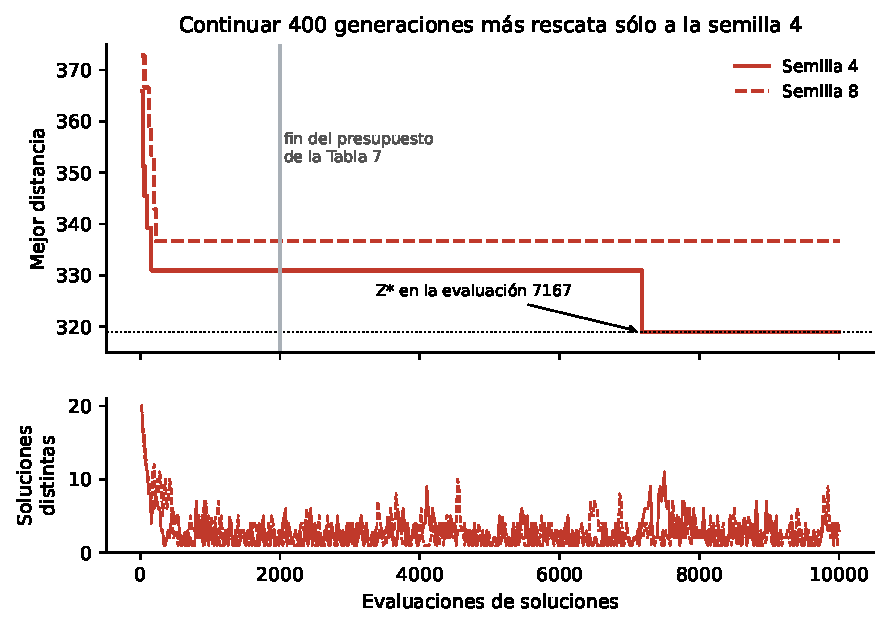
\includegraphics[width=.8\linewidth]{figuras/fig_semillas_extendidas.pdf}
\caption{Semillas 4 y 8 continuadas hasta 500 generaciones (10,000 evaluaciones). Las primeras 2,000 evaluaciones son idénticas a las de la Tabla~\ref{tab:individual}.}\label{fig:extendidas}
\end{figure}

Para separar el efecto del presupuesto, las dos semillas se continuaron hasta 500 generaciones; como la secuencia aleatoria es la misma, las primeras 100 generaciones coinciden con la corrida reportada (Figura~\ref{fig:extendidas}). La semilla 4 alcanzó el óptimo en la evaluación 7,167, generación 358; la semilla 8 no lo alcanzó en 10,000 evaluaciones. Por lo tanto, el estancamiento se explica por la combinación de una convergencia temprana alrededor de un óptimo local del vecindario de inversión y la pérdida de diversidad que impide abandonarlo. Ampliar el presupuesto rescata una de las dos corridas, pero con un costo cinco veces mayor que la corrida completa. La sección~\ref{sec:sens} muestra que una mayor tasa de mutación reduce estas fallas con el mismo presupuesto.

\section{Algoritmo de colonia de hormigas}

\subsection{Construcción probabilística y factibilidad}

ACO utiliza una memoria de feromonas y una preferencia heurística por distancias cortas, siguiendo el marco de Dorigo y Stützle (2004). Bullnheimer, Hartl y Strauss (1999) constituyen un antecedente de Ant System para ruteo de vehículos. La implementación de este trabajo es una adaptación sobre permutaciones con Split, no una reproducción de ese algoritmo publicado.

Cada hormiga parte del depósito y construye un orden de visita de los diez clientes sin repetirlos. Si \(U\) es el conjunto aún no seleccionado, la probabilidad de elegir \(j\in U\) desde \(i\) es
\begin{equation}\label{eq:prob}
p_{ij}=\frac{\tau_{ij}^{\alpha}\eta_{ij}^{\beta}}{\sum_{k\in U}\tau_{ik}^{\alpha}\eta_{ik}^{\beta}},\qquad \eta_{ij}=\frac{1}{c_{ij}}.
\end{equation}
Todas las distancias entre nodos diferentes son positivas en esta instancia. La hormiga \emph{no} es una construcción voraz capacitada: no vuelve al depósito cuando el vehículo se llena ni descarta clientes por capacidad remanente. Produce una permutación completa, un ``ciclo gigante'', y es Split quien decide dónde regresar al depósito y comprueba \(L_r\le 50\). Se elige esta variante para que GA y ACO compartan el mismo mecanismo de factibilidad y puedan explorar rutas parcialmente cargadas.

\textbf{Ejemplo de una hormiga.} La Tabla~\ref{tab:hormiga} reproduce la primera hormiga de la semilla 0, con toda la feromona en \(\tau_0=0.01\); en ese momento las probabilidades dependen sólo de la distancia. La demanda acumulada llega a 146, casi el triple de la capacidad, sin que la construcción lo impida.

\begin{table}[H]\centering\small
\caption{Construcción de la primera hormiga de la semilla 0 (\(\alpha=1\), \(\beta=2\), feromona inicial).}\label{tab:hormiga}
\begin{tabular}{rrlrrr}\toprule
Paso & Desde $i$ & Tres opciones más probables ($p_{ij}$) & Elegido & $p_{ij}$ & Demanda acumulada\\\midrule
1 & 1 & 10 (0.410), 11 (0.121), 7 (0.103) & 10 & 0.410 & 13\\
2 & 10 & 4 (0.197), 3 (0.142), 6 (0.142) & 7 & 0.096 & 33\\
3 & 7 & 6 (0.342), 8 (0.237), 11 (0.101) & 6 & 0.342 & 47\\
4 & 6 & 2 (0.355), 3 (0.185), 8 (0.115) & 2 & 0.355 & 59\\
5 & 2 & 3 (0.746), 4 (0.092), 11 (0.055) & 3 & 0.746 & 77\\
6 & 3 & 4 (0.457), 11 (0.190), 5 (0.163) & 4 & 0.457 & 87\\
7 & 4 & 5 (0.445), 11 (0.378), 9 (0.102) & 11 & 0.378 & 104\\
8 & 11 & 5 (0.482), 9 (0.348), 8 (0.169) & 5 & 0.482 & 119\\
9 & 5 & 9 (0.709), 8 (0.291) & 9 & 0.709 & 130\\
10 & 9 & 8 (1.000) & 8 & 1.000 & 146\\
\bottomrule\end{tabular}

\end{table}

La permutación resultante es \(\pi=(10,7,6,2,3,4,11,5,9,8)\). Split la divide en \((10,7)\,|\,(6,2,3)\,|\,(4,11)\,|\,(5,9,8)\), con cargas 33, 44, 27 y 42 y \(Z=355.668793\). En el paso 2 la hormiga eligió el cliente 7, que tenía probabilidad 0.096; la construcción es estocástica y no siempre toma el vecino más probable.

\subsection{Evaporación y refuerzo}\label{sec:feromona}

La feromona se evapora y recibe el refuerzo de las 20 hormigas de la iteración:
\begin{equation}\label{eq:tau}
\tau_{ij}^{t+1}=\max\{10^{-12},(1-\rho)\tau_{ij}^{t}\}+\sum_{h=1}^{20}\frac{Q_{\mathrm{ACO}}}{Z_h}a_{ij}^{h}.
\end{equation}
Aquí \(a_{ij}^h=1\) si los nodos \(i,j\) son consecutivos en el ciclo de la permutación completa de la hormiga, incluido el depósito al inicio y al final; vale cero en otro caso. El refuerzo es simétrico. El denominador \(Z_h\) corresponde a las rutas factibles decodificadas. El factor \(Q_{\mathrm{ACO}}=1\) es una escala de refuerzo y es distinto de la capacidad vehicular \(Q=50\).

\textbf{Adyacencias que Split separa.} La feromona aprende adyacencias del ciclo gigante, no arcos de las rutas. Cuando Split corta entre dos clientes consecutivos, esa adyacencia recibe refuerzo aunque el vehículo nunca recorra ese arco; a cambio, los arcos de regreso y salida del depósito que Split introduce entre una ruta y la siguiente no se refuerzan. Con cuatro rutas, 3 de las 11 adyacencias de cada ciclo son de este tipo. En las semillas 0--9, el 27.4\% de toda la feromona depositada (mínimo 25.9\%, máximo 29.5\% por iteración) cayó en adyacencias que no son arcos de las rutas decodificadas. La Tabla~\ref{tab:tau0} lo muestra al final de la semilla 0.

\begin{table}[H]\centering\small
\caption{Feromona final de la semilla 0 en las 11 adyacencias del mejor ciclo gigante \((10,4,5,11,9,8,7,6,2,3)\) y en los arcos del depósito que usan sus rutas sin ser adyacencias del ciclo.}\label{tab:tau0}
\begin{tabular}{lrl}\toprule
Par $\{i,j\}$ & $\tau_{ij}$ final & ¿Es arco de las rutas finales?\\\midrule
(1,10) & 0.2969 & Sí\\
(10,4) & 0.2894 & \textbf{No}: une el final de una ruta con el inicio de la siguiente\\
(4,5) & 0.2885 & Sí\\
(5,11) & 0.3023 & Sí\\
(11,9) & 0.2973 & \textbf{No}: une el final de una ruta con el inicio de la siguiente\\
(9,8) & 0.3038 & Sí\\
(8,7) & 0.3109 & Sí\\
(7,6) & 0.3110 & \textbf{No}: une el final de una ruta con el inicio de la siguiente\\
(6,2) & 0.3110 & Sí\\
(2,3) & 0.3107 & Sí\\
(3,1) & 0.2641 & Sí\\\midrule
(1,4) & 2.24e-02 & Sí, pero no es adyacencia del ciclo gigante\\
(1,6) & 2.75e-07 & Sí, pero no es adyacencia del ciclo gigante\\
(1,7) & 1.02e-04 & Sí, pero no es adyacencia del ciclo gigante\\
(1,9) & 1.14e-02 & Sí, pero no es adyacencia del ciclo gigante\\
(1,11) & 2.32e-03 & Sí, pero no es adyacencia del ciclo gigante\\
\bottomrule\end{tabular}

\end{table}

Las tres adyacencias separadas, \((10,4)\), \((11,9)\) y \((7,6)\), terminan con tanta feromona como los arcos recorridos (0.289 a 0.311), mientras que los arcos del depósito recorridos por las rutas quedan entre \(2.8\times10^{-7}\) y 0.022. Esto tiene dos efectos. Primero, la feromona describe el \emph{orden de concatenación} de las rutas dentro del ciclo, no la red de arcos usada: refuerza, por ejemplo, que la ruta que termina en 7 vaya seguida de la que empieza en 6. Esto es coherente con la representación, porque ese orden es lo que Split necesita para volver a producir la misma solución. Segundo, una misma solución puede escribirse como muchos ciclos gigantes distintos (cambiando el orden y el sentido de sus rutas), y la colonia refuerza sólo uno de ellos; las demás escrituras pierden probabilidad aunque decodifiquen lo mismo. En esta instancia esto no impidió llegar al óptimo, pero significa que la feromona no puede interpretarse como una medida de la calidad de cada arco.

\textbf{Piso numérico y ausencia de cota superior.} Un arco que nunca se refuerza vale \(\tau_0(1-\rho)^t\). Con \(\rho=0.2\) y 100 iteraciones llega a \(0.01\times0.8^{100}=2.04\times10^{-12}\), por encima de \(10^{-12}\): en el experimento principal el piso nunca se activó. Con \(\rho=0.5\) se activa desde la iteración 34 (4,174 activaciones en la semilla 0). El piso es una protección numérica para corridas largas o con evaporación alta; no es un mecanismo de exploración, porque la razón entre la feromona máxima y \(10^{-12}\) supera \(3\times10^{11}\), y un arco en el piso tiene probabilidad prácticamente nula. No hay cota superior explícita, pero sí una implícita: cada hormiga deposita a lo más \(1/Z^*\) en un par por iteración, de modo que
\begin{equation}\label{eq:cota}
\tau_{ij}^t\le \tau_0(1-\rho)^t+\frac{20}{\rho\,Z^*}\approx 0.3135 .
\end{equation}
La feromona máxima final osciló entre 0.3110 y 0.3132, prácticamente en esa cota (Figura~\ref{fig:feromona}).

\begin{figure}[H]\centering
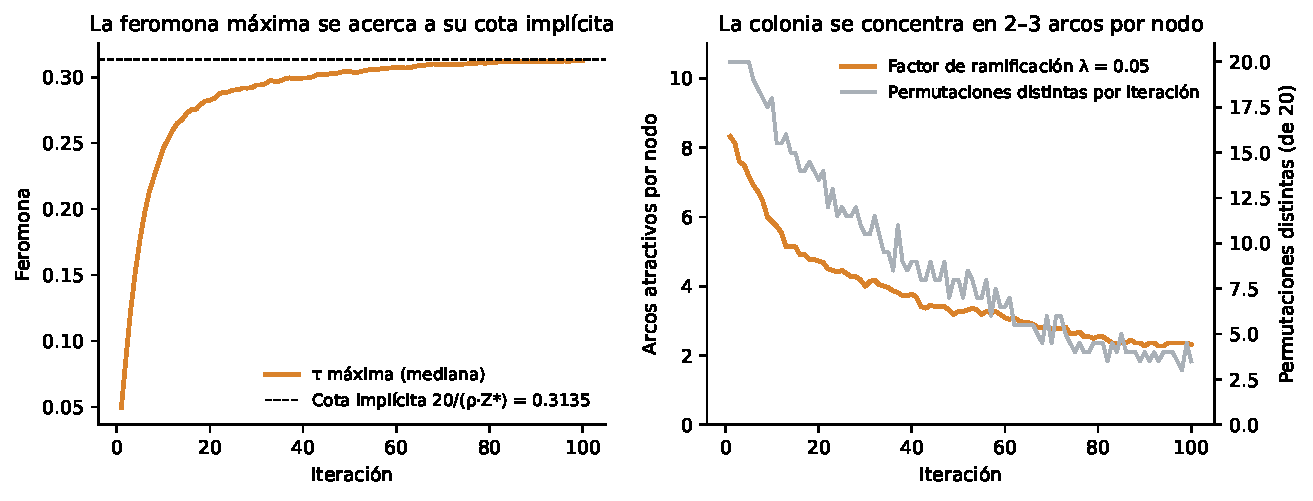
\includegraphics[width=\linewidth]{figuras/fig_feromona.pdf}
\caption{Dinámica de la feromona en las semillas 0--9 (mediana): feromona máxima frente a la cota~\eqref{eq:cota}, factor de ramificación \(\lambda=0.05\) y permutaciones distintas construidas en cada iteración.}\label{fig:feromona}
\end{figure}

\textbf{Concentración.} El factor de ramificación \(\lambda\) (Gambardella y Dorigo, 1995) cuenta cuántos arcos de cada nodo tienen feromona mayor que \(\min+0.05(\max-\min)\). Bajó de 8.3 arcos por nodo en la primera iteración a 2.3 en la última, y las 20 hormigas de la última iteración construyeron entre 1 y 5 permutaciones distintas. Al final de la semilla 0, una hormiga reconstruye exactamente el mejor ciclo con probabilidad 0.774. La colonia sí se concentra en exceso: en las últimas 40 iteraciones construye, en mediana, entre 3 y 7 permutaciones distintas por iteración, y casi todas repiten el mismo ciclo. En CVRP\_10 esto no causó fallas porque el óptimo se encuentra antes de la concentración (sección~\ref{sec:convergencia}). En la instancia adicional E10-b sí aparecieron fallas (sección~\ref{sec:instancias}). Un ensayo exploratorio que impone \(\tau_{ij}\ge r\max\tau\), en el espíritu de MAX--MIN Ant System (Stützle y Hoos, 2000), subió los éxitos en E10-b de 16/30 a 19, 25 y 26/30 con \(r=0.01\), \(0.05\) y \(0.1\), sin cambiar CVRP\_10 (30/30 en todos los casos). Ese mecanismo no forma parte de la configuración evaluada.

\Needspace{14\baselineskip}
\subsection{Hiperparámetros y pseudocódigo}

\begin{table}[H]\centering\small
\caption{Configuración principal de ACO.}\label{tab:acoparam}
\begin{tabular}{p{3.2cm}p{2.6cm}p{8.8cm}}\toprule
Parámetro & Valor & Justificación\\\midrule
Hormigas & 20 & Igual al tamaño de población del GA: 20 construcciones por actualización.\\
Iteraciones & 100 & \(20\times100=2000\) soluciones evaluadas, igual presupuesto que GA.\\
\(\alpha\) & 1 & Influencia lineal de la feromona, valor estándar en Ant System (Dorigo y Stützle, 2004).\\
\(\beta\) & 2 & Preferencia por clientes cercanos; en la sensibilidad, \(\beta=0\) falla y \(\beta\ge1\) funciona.\\
\(\rho\) & 0.20 & Una adyacencia sin refuerzo pierde la mitad de su feromona en 3 iteraciones.\\
\(Q_{\mathrm{ACO}}\) & 1 & Escala común para depositar \(1/Z_h\).\\
\(\tau_0\) & 0.01 & Todas las transiciones comienzan con igual peso positivo.\\
Piso numérico & \(10^{-12}\) & Evita pesos nulos; inactivo con \(\rho=0.2\) en 100 iteraciones (sección~\ref{sec:feromona}).\\
Semillas & 0--9 & Diez ejecuciones independientes.\\
Búsqueda local & Ninguna & La capacidad y las divisiones se resuelven con Split.\\\bottomrule
\end{tabular}
\end{table}

Los valores principales se fijaron antes del experimento, a partir de los valores usuales de Ant System, y no se cambiaron después. La sección~\ref{sec:sensaco} evalúa todas sus combinaciones con \(\alpha\), \(\beta\), \(\rho\) y el número de hormigas.

\Needspace{17\baselineskip}
\begin{lstlisting}[caption={Pseudocódigo de ACO con decodificación Split.}]
Inicializar toda feromona en 0.01 y mejor costo en infinito
Repetir 100 iteraciones:
    Para cada una de 20 hormigas:
        Partir del deposito; marcar todos los clientes como no visitados
        Elegir clientes sin repeticion segun feromona^alpha / distancia^beta
            (sin revisar capacidad: se construye el ciclo gigante completo)
        Aplicar Split a la permutacion completa                 (1 evaluacion)
        Guardar costo y rutas; actualizar la mejor solucion acumulada
    Evaporar feromonas: max(1e-12, 0.8 * tau)
    Para cada hormiga:
        Depositar 1/costo en ambas direcciones de cada adyacencia
        de su ciclo de permutacion (incluidas las conexiones al deposito)
    Registrar el mejor costo acumulado
Devolver la mejor solucion y su historial
\end{lstlisting}

\Needspace{12\baselineskip}
\subsection{Validación y trazado de rutas}

ACO alcanzó el óptimo en las diez semillas principales. En todas obtuvo cuatro rutas y 27\% de capacidad global libre. La Tabla~\ref{tab:rutasaco} muestra la semilla 0, que coincide con la mejor solución del GA salvo el orden de presentación y el sentido de algunas rutas.

\begin{table}[H]\centering\small
\caption{Rutas de ACO + Split, semilla 0.}\label{tab:rutasaco}
\begin{tabular}{llrrr}\toprule
Ruta & Recorrido & Distancia & Carga / 50 & Libre (\%)\\\midrule
R1 & \(1\to10\to1\) & 22.360680 & 13 & 74\\
R2 & \(1\to3\to2\to6\to1\) & 101.187844 & 44 & 12\\
R3 & \(1\to4\to5\to11\to1\) & 86.184637 & 42 & 16\\
R4 & \(1\to7\to8\to9\to1\) & 109.256327 & 47 & 6\\\bottomrule
\end{tabular}
\end{table}

\begin{figure}[H]\centering
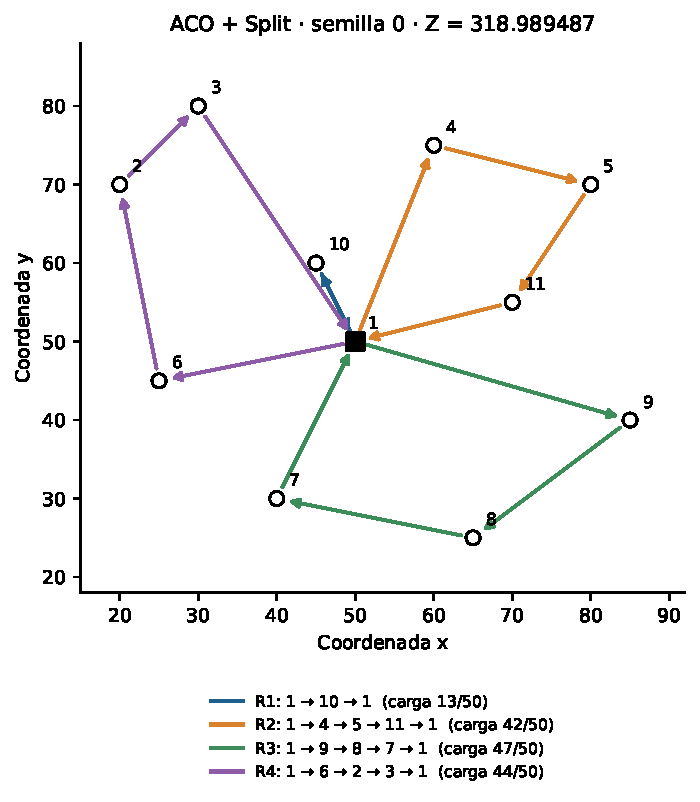
\includegraphics[width=.62\linewidth]{figuras/fig2_rutas_aco.pdf}
\caption{Mejor solución de ACO (semilla 0). Se conserva la misma escala y los mismos colores por ruta que en la Figura~\ref{fig:rutasga}.}\label{fig:rutasaco}
\end{figure}

La coincidencia de las Figuras~\ref{fig:rutasga} y~\ref{fig:rutasaco} indica que ambos métodos pueden recuperar la misma agrupación óptima. No indica que sigan el mismo proceso de búsqueda: GA recombina individuos, mientras ACO modifica probabilidades mediante feromonas. La sección~\ref{sec:convergencia} compara su diversidad y su velocidad de convergencia.

\section{Comparación integral con la etapa 1}

\subsection{Protocolo y comprobaciones}\label{sec:protocolo}

Las cuatro implementaciones se ejecutaron el 20 de octubre de 2026 en el mismo equipo, con procesador Intel Core i7-13620H, Windows 11, Python 3.12.14, PuLP 3.3.0 y CBC 2.10.3. Se realizó un calentamiento por método; después, diez repeticiones, rotando el orden de ejecución de los cuatro métodos. Para GA y ACO se usaron semillas 0 a 9; el calentamiento empleó 999. No se suministró el óptimo a la búsqueda ni se utilizó como criterio de paro.

El método exacto conserva la formulación principal de flujo de producto de la etapa 1: 110 variables binarias de recorrido, 110 continuas de carga y 154 restricciones. Las visitas únicas, la conservación de recorrido, el balance de carga, el vínculo \(0\le f_{ij}\le Qx_{ij}\) y los regresos vacíos garantizan rutas factibles y conectadas para demandas positivas. Se ejecutó CBC con \texttt{threads=0}, brechas relativa y absoluta cero y límite de 120 s. En las diez llamadas se obtuvo optimalidad probada. La heurística conserva las fusiones de Clarke--Wright y la búsqueda 2-opt de la etapa anterior.

\textbf{Qué se cronometra.} Los intervalos se midieron con \texttt{time.perf\_counter()}. Para el exacto se incluyen construcción, solución y reconstrucción; para CW+2-opt, ahorros, fusiones y mejora; para GA y ACO, inicialización, búsqueda, decodificación final e historial. Quedan fuera del cronometraje la lectura de la instancia, el cálculo de la matriz de distancias, las verificaciones de factibilidad, la certificación por subconjuntos y las figuras. El mismo número de evaluaciones de GA y ACO controla su esfuerzo de búsqueda, pero no implica el mismo trabajo por evaluación ni el mismo tiempo; por eso las comparaciones se reportan por separado en evaluaciones (sección~\ref{sec:convergencia}) y en tiempo real (sección~\ref{sec:tiempos}).

\textbf{Pruebas automatizadas.} La validación se implementó como pruebas en \texttt{tests/test\_etapa2.py}, que se ejecutan con \texttt{python -m pytest -q tests} (5 pruebas, alrededor de 1.3 s). Los casos no se eligen a mano: las 50 permutaciones de Split y los 1,000 cruces OX se generan con \texttt{random.Random(2026)}, una semilla distinta de las experimentales. Las pruebas comprueban lo siguiente:
\begin{enumerate}
\item \textbf{Caso fijo verificable.} Para \(\pi=(4,5,11,6,2,3,10,7,8,9)\) (sección~\ref{sec:ejsplit}), Split devuelve las cuatro rutas óptimas y su costo coincide con el mínimo de las 512 combinaciones de cortes.
\item \textbf{Split contra 512 cortes.} Para cada una de las 50 permutaciones, el costo de Split coincide con el mínimo de las 512 combinaciones (tolerancia \(10^{-9}\)), y Split no reordena los clientes.
\item \textbf{Operadores.} En 1,000 cruces OX seguidos de una inversión, el hijo es siempre una permutación de \(\{2,\dots,11\}\).
\item \textbf{Óptimo independiente.} Una programación dinámica por subconjuntos (Held--Karp por ruta y partición de conjuntos) obtiene \(Z^*=318.9894867478301\) y los grupos \(\{2,3,6\},\{4,5,11\},\{7,8,9\},\{10\}\).
\item \textbf{Soluciones finales, incluidas las no óptimas.} Para las semillas 0--9 de GA y ACO se verifican cobertura única, salida y regreso al depósito, capacidad, coincidencia entre el costo reportado y la suma de arcos, historial no creciente y los valores de la Tabla~\ref{tab:individual}.
\end{enumerate}

\subsection{Calidad, brechas y utilización}

Para cualquier método \(M\) se calculan la brecha respecto al óptimo y la mejora respecto a la heurística anterior:
\begin{equation}\label{eq:gap}
\mathrm{GAP}_Z(M)=100\,\frac{Z_M-Z^*}{Z^*},\qquad I_{\mathrm{CW}}(M)=100\,\frac{Z_{\mathrm{CW}}-Z_M}{Z_{\mathrm{CW}}}.
\end{equation}
Las bases de ambos porcentajes son distintas. Un GAP positivo indica distancia adicional; un \(I_{\mathrm{CW}}\) positivo indica reducción frente a Clarke--Wright. En las comparaciones de promedios se sustituye \(Z_M\) por la distancia media de las diez corridas.

\begin{table}[H]\centering\small
\caption{Calidad de las diez ejecuciones por método.}\label{tab:calidad}
\begin{tabular}{lrrrrr}\toprule
Método & Mejor \(Z\) & Media \(Z\) & Peor \(Z\) & GAP medio (\%) & Óptimos\\\midrule
Exacto & 318.989487 & 318.989487 & 318.989487 & 0.000 & 10/10\\
CW+2opt & 339.252870 & 339.252870 & 339.252870 & 6.352 & 0/10\\
GA & 318.989487 & 321.958694 & 336.713769 & 0.931 & 8/10\\
ACO & 318.989487 & 318.989487 & 318.989487 & 0.000 & 10/10\\\bottomrule
\end{tabular}
\end{table}

GA tuvo un GAP medio de 0.931\%, mientras ACO tuvo 0\%. La mejora media frente a CW+2-opt fue 5.098\% para GA y 5.973\% para ACO; la mejor corrida de ambos mejoró 5.973\%. La desviación estándar muestral de la distancia fue 6.405001 para GA y prácticamente cero para ACO. Los dos fallos de GA correspondieron a las semillas 4 y 8, con 330.957278 y 336.713769 unidades; sus rutas y la causa del estancamiento se analizan en la sección~\ref{sec:diversidad}.

Los cuatro métodos produjeron cuatro rutas en todas las ejecuciones principales. En consecuencia, todos tuvieron 73\% de utilización y 27\% de espacio libre global. La igualdad de ocupación no implica igualdad de distancia: la asignación de clientes explica el GAP de CW+2-opt y de las dos corridas no óptimas del GA.

\begin{table}[H]\centering\small
\caption{Resultados individuales de GA y ACO (semillas 0--9). La primera evaluación con \(Z^*\) proviene de la copia instrumentada (sección~\ref{sec:convergencia}).}\label{tab:individual}
\begin{tabular}{rrrrrrr}\toprule
Semilla & \(Z_{\mathrm{GA}}\) & \(t_{\mathrm{GA}}\) (ms) & 1.ª eval. con \(Z^*\), GA & \(Z_{\mathrm{ACO}}\) & \(t_{\mathrm{ACO}}\) (ms) & 1.ª eval. con \(Z^*\), ACO\\\midrule
0 & 318.989487 & 31.240 & 796 & 318.989487 & 56.242 & 40\\
1 & 318.989487 & 27.737 & 660 & 318.989487 & 54.738 & 75\\
2 & 318.989487 & 29.884 & 161 & 318.989487 & 56.608 & 35\\
3 & 318.989487 & 30.481 & 610 & 318.989487 & 84.443 & 38\\
4 & 330.957278 & 28.460 & -- & 318.989487 & 58.069 & 25\\
5 & 318.989487 & 29.605 & 1212 & 318.989487 & 57.451 & 39\\
6 & 318.989487 & 29.136 & 329 & 318.989487 & 54.673 & 20\\
7 & 318.989487 & 29.849 & 371 & 318.989487 & 56.387 & 2\\
8 & 336.713769 & 29.401 & -- & 318.989487 & 56.790 & 60\\
9 & 318.989487 & 29.752 & 423 & 318.989487 & 57.840 & 28\\\bottomrule
\end{tabular}
\end{table}

\Needspace{14\baselineskip}
\subsection{Convergencia por evaluaciones y diversidad de la búsqueda}\label{sec:convergencia}

\begin{figure}[H]\centering
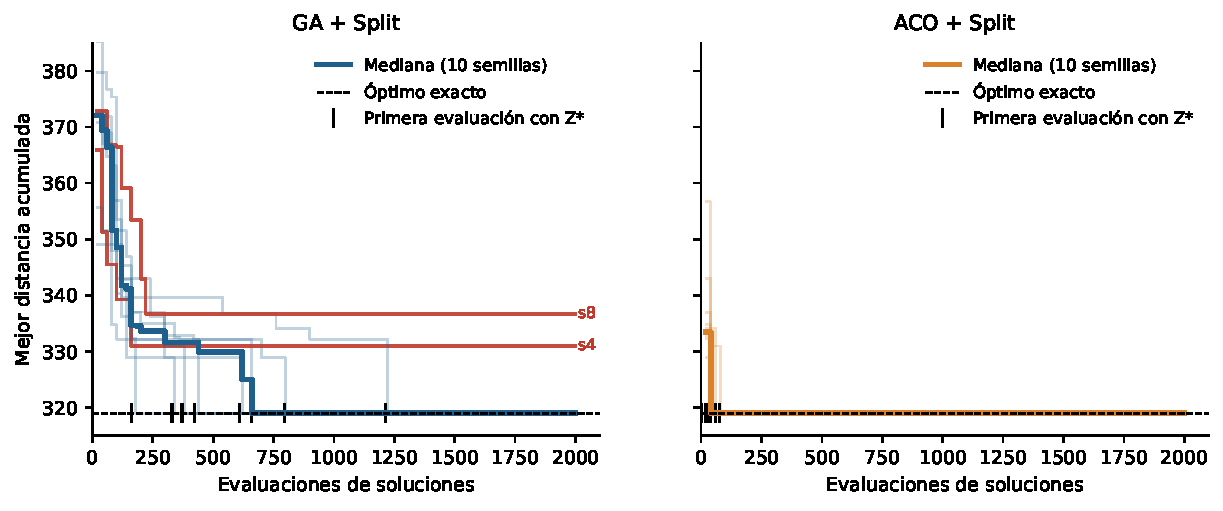
\includegraphics[width=\linewidth]{figuras/fig3_convergencia.pdf}
\caption{Convergencia de las diez corridas. Las curvas tenues son ejecuciones individuales, la curva gruesa es la mediana y las marcas verticales indican la primera evaluación en que cada semilla alcanza \(Z^*\). En rojo, las semillas 4 y 8 del GA.}\label{fig:convergencia}
\end{figure}

La Figura~\ref{fig:convergencia} usa evaluaciones de soluciones como eje común. En el GA, la primera evaluación con \(Z^*\) varía de 161 a 1,212 entre las ocho semillas exitosas; en ACO, de 2 a 75. La mediana del GA llega al óptimo, pero dos curvas individuales terminan por encima; la mediana por sí sola ocultaría esos fallos. La estabilización de una curva describe el mejor resultado observado y no constituye una demostración de optimalidad; esa comprobación proviene del método exacto.

Diez semillas dan una distribución muy gruesa, por lo que la medición se amplió a las semillas 0--99 con la misma configuración (Figura~\ref{fig:primera}). El GA alcanzó \(Z^*\) en 86 de 100 corridas dentro de las 2,000 evaluaciones, con mediana de 370.5 evaluaciones y rango intercuartil de 217 a 643.5. ACO lo alcanzó en las 100, con mediana de 37 evaluaciones (rango intercuartil de 26 a 49.5) y nunca después de la evaluación 100, es decir, dentro de sus primeras cinco iteraciones. Por evaluaciones, ACO llega al óptimo unas diez veces antes que GA en esta instancia.

\begin{figure}[H]\centering
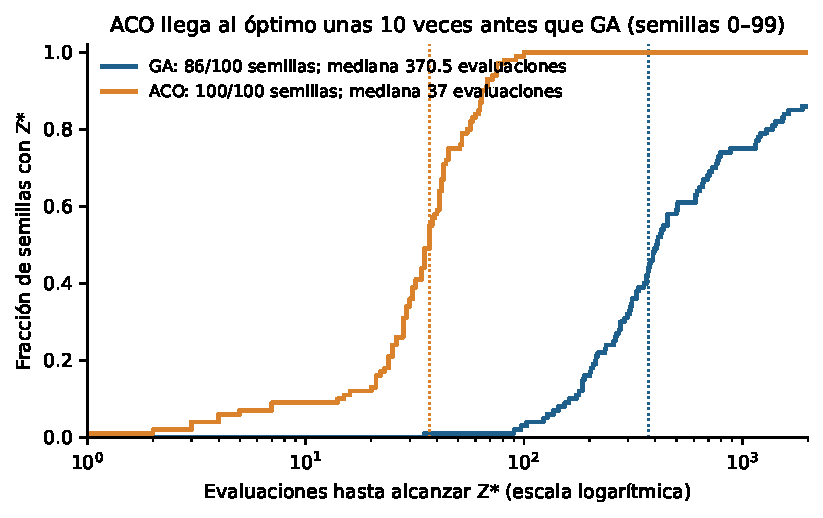
\includegraphics[width=.75\linewidth]{figuras/fig_primera_evaluacion.pdf}
\caption{Distribución de la primera evaluación con \(Z^*\) en 100 semillas (curva de tiempo de ejecución, Hoos y Stützle, 2004). Las líneas punteadas son las medianas.}\label{fig:primera}
\end{figure}

\textbf{Por qué coinciden las soluciones pero no las búsquedas.} La Figura~\ref{fig:diversidad} (derecha) compara la diversidad de permutaciones. La población del GA pierde diversidad bruscamente en las primeras 400 evaluaciones (de 0.80 a cerca de 0.10) y después varía según la semilla. La colonia la pierde de forma gradual (de 0.72 a 0.05 en 2,000 evaluaciones). La velocidad de ACO, sin embargo, no proviene del aprendizaje por feromona: el óptimo aparece cuando la feromona todavía es casi uniforme, guiado por la información heurística \(\eta^\beta\). Un control con \(\alpha=0\), en el que la feromona no interviene, también alcanzó el óptimo en 30 de 30 semillas, con mediana de 44 evaluaciones frente a 34 con \(\alpha=1\). En CVRP\_10, el trabajo de ACO lo hace principalmente su construcción probabilística orientada por distancia, mientras que el GA debe descubrir la agrupación por selección, cruza y mutación desde permutaciones aleatorias.

\Needspace{14\baselineskip}
\subsection{Tiempos y compromiso entre calidad y rapidez}\label{sec:tiempos}

La reducción temporal relativa al exacto se calcula con los tiempos medios de la ejecución del 20 de octubre:
\begin{equation}\label{eq:rt}
R_t(M)=100\,\frac{t_E-t_M}{t_E}.
\end{equation}

\begin{table}[H]\centering\small
\caption{Tiempos de ejecución, en milisegundos (Intel Core i7-13620H, Windows 11, Python 3.12.14).}\label{tab:tiempos}
\begin{tabular}{lrrrr}\toprule
Método & Media & Desv. est. & Mediana & \(R_t\) (\%)\\\midrule
Exacto & 2162.488 & 27.729 & 2164.204 & 0.0000\\
CW+2opt & 0.116 & 0.021 & 0.110 & 99.9947\\
GA & 29.555 & 0.980 & 29.679 & 98.6333\\
ACO & 59.324 & 8.900 & 56.699 & 97.2567\\\bottomrule
\end{tabular}
\end{table}

El genético tardó aproximadamente 29.555 ms y ACO, 59.324 ms, con el mismo número de evaluaciones: cada evaluación de ACO cuesta cerca del doble. CW+2-opt fue el método más rápido, con 0.116 ms, a cambio de una brecha de 6.352\%. El exacto necesitó 2162.488 ms en promedio y aportó la certificación de optimalidad. Las desviaciones estándar y medianas se calculan sobre diez observaciones por método, sin eliminar corridas lentas.

\textbf{Costo por evaluación.} Para explicar la diferencia se cronometró por separado cada componente en una copia de los algoritmos con relojes internos. Esta medición se hizo en otro equipo (x86\_64, Linux, Python 3.13.16), donde las corridas completas tardaron 31.4 ms (GA) y 59.5 ms (ACO), valores cercanos a los de la Tabla~\ref{tab:tiempos}. En el GA, Split ocupa el 55.2\% del tiempo, la selección, cruza y mutación el 42.6\% y el reemplazo el 2.3\%. En ACO, la construcción de las hormigas ocupa el 61.1\%, Split el 29.3\% y la actualización de feromona el 9.5\%. La construcción calcula en cada paso un peso por cada cliente no visitado, lo que explica que una evaluación de ACO cueste unos 29.8 \(\mu\)s frente a 15.7 \(\mu\)s en el GA. Por eso igualar evaluaciones no iguala el tiempo de cómputo.

\textbf{Tiempo real hasta el óptimo.} Medido en ese mismo equipo, el GA alcanzó \(Z^*\) entre 2.9 y 24.1 ms después de iniciar en sus ocho semillas exitosas, y ACO entre 0.08 y 3.4 ms. Aunque cada evaluación de ACO es más cara, ACO llega antes al óptimo también en tiempo, porque necesita unas diez veces menos evaluaciones. Estas cifras dependen del equipo y deben volver a medirse en el equipo del experimento principal si se desea reportarlas junto con la Tabla~\ref{tab:tiempos}.

\begin{figure}[H]\centering
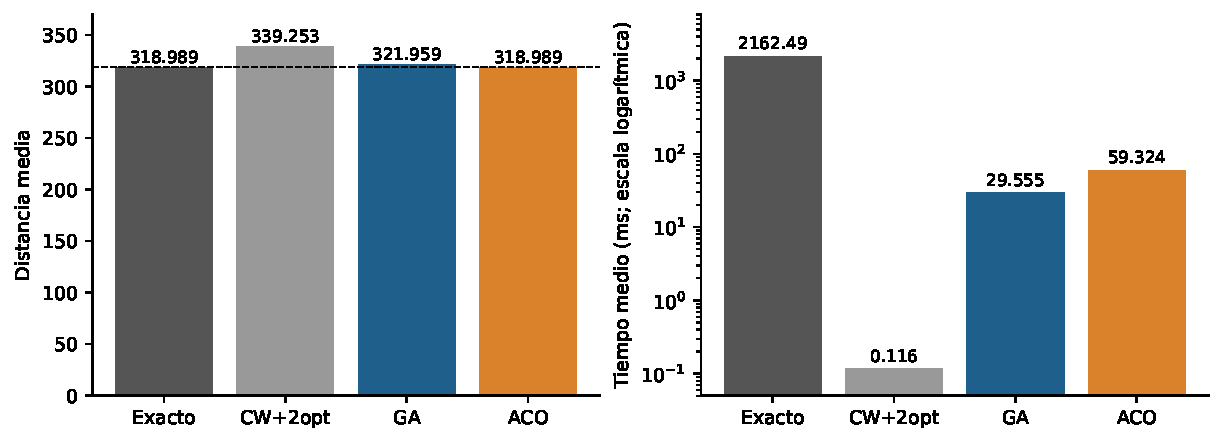
\includegraphics[width=\linewidth]{figuras/fig4_distancia_tiempo.pdf}
\caption{Distancia y tiempo medios de los cuatro métodos, medidos el 20 de octubre de 2026. La línea discontinua indica el óptimo de distancia.}\label{fig:disttiempo}
\end{figure}

El panel izquierdo de la Figura~\ref{fig:disttiempo} compara distancias medias, por lo que distingue el mejor resultado posible del desempeño habitual del GA. El panel derecho usa escala logarítmica para mostrar tiempos separados por varios órdenes de magnitud. Cada etiqueta corresponde a la media de la Tabla~\ref{tab:tiempos}.

En la etapa 1 se reportaron 2975.400 ms para el exacto y 0.198 ms para la heurística. Se conservan como antecedentes de otra ejecución; las tablas y porcentajes de esta etapa usan exclusivamente las mediciones nuevas. Las diferencias temporales pueden depender de versión de Python, carga del equipo y variación de ejecución; no se atribuyen a una mejora del modelo porque éste se mantuvo igual.

\textbf{Alcance de los tiempos.} Las cifras describen CVRP\_10 con diez clientes y no deben extrapolarse a instancias grandes. El costo de Split crece aproximadamente con \(n\) por la longitud máxima de una ruta, la construcción de ACO con \(n^2\) por hormiga, y el modelo exacto de forma combinatoria. En las instancias de 20 y 30 clientes de la sección~\ref{sec:instancias}, una corrida de ACO con 2,000 evaluaciones tardó 204 y 344 ms en el equipo Linux, frente a 66 y 70 ms del GA.

\section{Sensibilidad y alcance de los resultados}\label{sec:sens}

\subsection{Ensayo inicial}

La versión entregada incluyó una comprobación que cambiaba un parámetro a la vez: \(p_m\in\{0.1,0.2,0.4\}\) para GA y \(\rho\in\{0.1,0.2,0.5\}\) para ACO, con el presupuesto de 2,000 evaluaciones y las mismas diez semillas nuevas, 100--109, para una comparación emparejada. Se volvió a ejecutar y los resultados coinciden exactamente (Tabla~\ref{tab:sensini}).

\begin{table}[H]\centering\small
\caption{Ensayo inicial: diez semillas adicionales (100--109) por configuración.}\label{tab:sensini}
\begin{tabular}{llrrr}\toprule
Método & Parámetro & Media \(Z\) & Peor \(Z\) & Óptimos\\\midrule
GA & \(p_m=0.1\) & 320.309230 & 332.186915 & 9/10\\
GA & \(p_m=0.2\) & 324.475216 & 336.713769 & 6/10\\
GA & \(p_m=0.4\) & 318.989487 & 318.989487 & 10/10\\
ACO & \(\rho=0.1\) & 318.989487 & 318.989487 & 10/10\\
ACO & \(\rho=0.2\) & 318.989487 & 318.989487 & 10/10\\
ACO & \(\rho=0.5\) & 318.989487 & 318.989487 & 10/10\\\bottomrule
\end{tabular}
\end{table}

Con diez semillas, la relación entre \(p_m\) y el éxito no fue monótona (9, 6 y 10 éxitos), y la configuración principal obtuvo 8/10 con las semillas 0--9 y 6/10 con las 100--109. Diez semillas no bastan para separar estas configuraciones, por lo que el ensayo se amplió en tres direcciones.

\subsection{Algoritmo genético: mutación, población y cruza}

Se evaluaron \(p_m\in\{0,0.1,0.2,0.4,0.6,0.8,1\}\) con poblaciones de 10, 20 y 40 individuos, manteniendo 2,000 evaluaciones (199, 99 y 49 generaciones), con 100 semillas nuevas (300--399) por configuración. La Tabla~\ref{tab:sensga} reporta las corridas que alcanzan \(Z^*\) y su intervalo de confianza de Wilson al 95\% (Wilson, 1927).

\begin{table}[H]\centering\small
\caption{GA en CVRP\_10: corridas con \(Z^*\) de 100 e intervalo de Wilson al 95\% (\%), \(p_c=0.9\). En negritas, la configuración principal.}\label{tab:sensga}
\begin{tabular}{lccc}\toprule
$p_m$ & Población 10 (199 gen.) & Población 20 (99 gen.) & Población 40 (49 gen.)\\\midrule
0 & 1 [0, 5] & 19 [13, 28] & 62 [52, 71]\\
0.1 & 57 [47, 66] & 72 [63, 80] & 80 [71, 87]\\
0.2 & 69 [59, 77] & \textbf{80 [71, 87]} & 96 [90, 98]\\
0.4 & 82 [73, 88] & 94 [88, 97] & 97 [92, 99]\\
0.6 & 95 [89, 98] & 99 [95, 100] & 95 [89, 98]\\
0.8 & 98 [93, 99] & 99 [95, 100] & 92 [85, 96]\\
1 & 99 [95, 100] & 95 [89, 98] & 92 [85, 96]\\
\bottomrule\end{tabular}

\end{table}

\begin{figure}[H]\centering
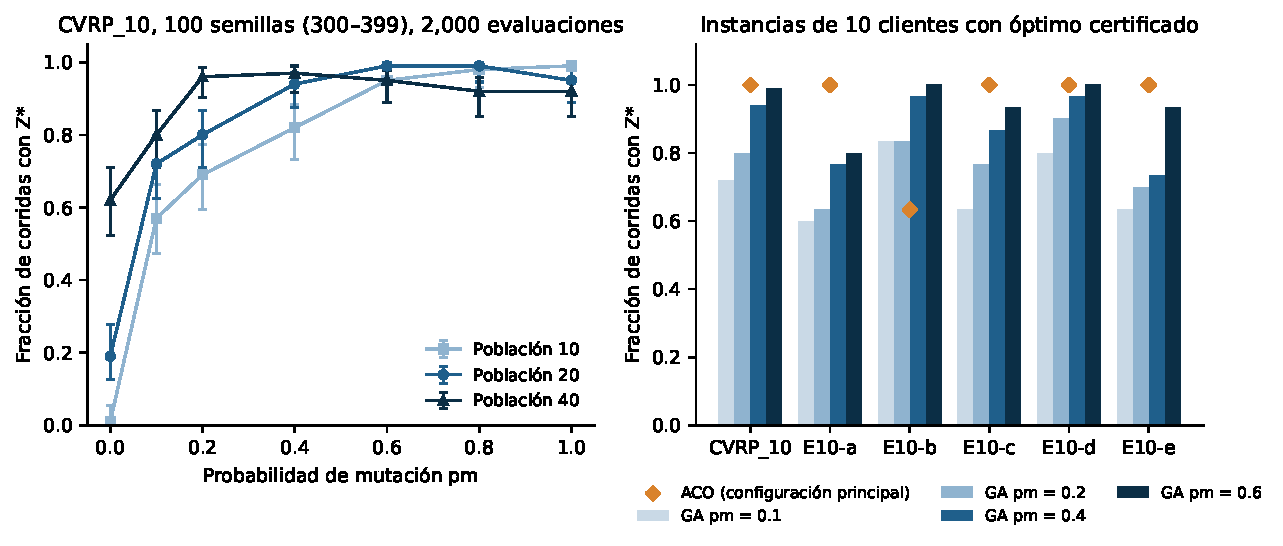
\includegraphics[width=\linewidth]{figuras/fig_sensibilidad_ga.pdf}
\caption{Izquierda: fracción de corridas con \(Z^*\) según \(p_m\) y tamaño de población (barras: intervalo de Wilson al 95\%). Derecha: GA con distintas \(p_m\) y ACO en CVRP\_10 (100 semillas) y en las cinco instancias adicionales (30 semillas).}\label{fig:sensga}
\end{figure}

Con 100 semillas, la configuración principal (\(p_m=0.2\), población 20) alcanzó el óptimo en 80 corridas, con intervalo de 71\% a 87\%, y \(p_m=0.4\) en 94, con intervalo de 88\% a 97\%. Los intervalos apenas se tocan, por lo que la ventaja de 0.4 se mantiene en esta instancia; con \(p_m=0.6\) y 0.8 se obtuvieron 99 éxitos. Sin mutación, sólo 19 corridas llegaron al óptimo: la inversión es el principal mecanismo de exploración una vez que la población converge, en línea con la sección~\ref{sec:diversidad}. Una población de 40 con \(p_m=0.2\) alcanzó 96 éxitos, a cambio de menos generaciones. La probabilidad de cruza tuvo un efecto menor (Tabla~\ref{tab:sensgapc}).

\begin{table}[H]\centering\small
\caption{GA en CVRP\_10 con población 20: efecto de \(p_c\) (100 semillas, 300--399).}\label{tab:sensgapc}
\begin{tabular}{lrrrr}\toprule
$p_c$ & Éxitos, $p_m=0.2$ & Media $Z$ & Éxitos, $p_m=0.4$ & Media $Z$\\\midrule
0.5 & 76/100 & 322.473 & 90/100 & 320.305\\
0.7 & 72/100 & 322.957 & 96/100 & 319.596\\
0.9 & 80/100 & 321.844 & 94/100 & 319.905\\
1 & 81/100 & 321.731 & 95/100 & 319.632\\
\bottomrule\end{tabular}

\end{table}

\subsection{Colonia de hormigas: sensibilidad conjunta}\label{sec:sensaco}

Se ejecutó un diseño factorial completo con \(\alpha\in\{0.5,1,2\}\), \(\beta\in\{0,1,2,5\}\), \(\rho\in\{0.1,0.2,0.5\}\) y 10, 20 o 40 hormigas (200, 100 o 50 iteraciones, siempre 2,000 evaluaciones), con 30 semillas (200--229) por combinación: 108 configuraciones y 3,240 corridas. Como casi todas las configuraciones alcanzan el óptimo con 2,000 evaluaciones, se reportan también los éxitos con sólo 200 evaluaciones y la mediana de evaluaciones hasta \(Z^*\), que sí distinguen las configuraciones.

\begin{table}[H]\centering\small
\caption{ACO en CVRP\_10 por \(\alpha\) y \(\beta\), combinando los tres valores de \(\rho\) y de hormigas (270 corridas por celda). Cada celda: corridas con \(Z^*\) en 2,000 evaluaciones · corridas con \(Z^*\) en 200 · mediana de evaluaciones hasta \(Z^*\).}\label{tab:sensaco}
\begin{tabular}{lcccc}\toprule
 & $\beta=0$ & $\beta=1$ & $\beta=2$ & $\beta=5$\\\midrule
$\alpha=0.5$ & 38/270 · 0 · 1499 & 270/270 · 69 · 285 & 270/270 · 269 · 40 & 270/270 · 270 · 4.5\\
$\alpha=1$ & 58/270 · 8 · 1254 & 270/270 · 237 · 117 & \textbf{270/270 · 270 · 35.5} & 270/270 · 270 · 4.5\\
$\alpha=2$ & 14/270 · 3 · 352.5 & 239/270 · 237 · 69 & 267/270 · 267 · 27 & 270/270 · 270 · 4.5\\
\bottomrule\end{tabular}

\end{table}

\begin{figure}[H]\centering
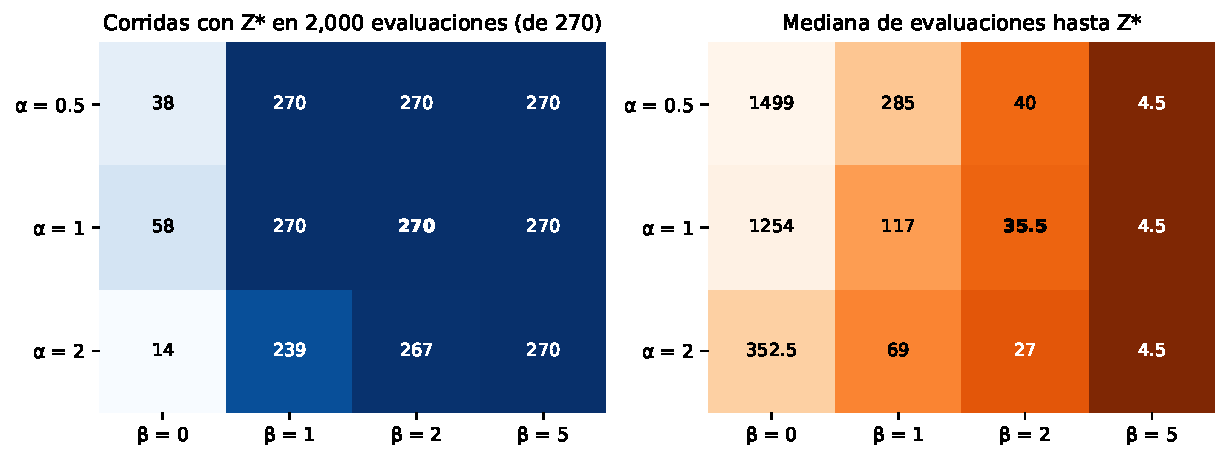
\includegraphics[width=\linewidth]{figuras/fig_sensibilidad_aco.pdf}
\caption{Sensibilidad de ACO a \(\alpha\) y \(\beta\). En negritas, la configuración principal.}\label{fig:sensaco}
\end{figure}

El parámetro dominante es \(\beta\) (Tabla~\ref{tab:sensaco} y Figura~\ref{fig:sensaco}). Sin información heurística (\(\beta=0\)) sólo 110 de 810 corridas alcanzan el óptimo; con \(\beta=2\), 807; con \(\beta=5\), las 810, con mediana de 4.5 evaluaciones. En esta instancia, la preferencia por vecinos cercanos por sí sola orienta a la colonia hacia la agrupación óptima. Hay interacción entre \(\alpha\) y \(\beta\): con \(\beta\le1\), \(\alpha=2\) empeora los resultados (14/270 con \(\beta=0\) y 239/270 con \(\beta=1\)) porque la feromona domina antes de acumular información útil; con \(\beta\ge2\), \(\alpha\) acelera la convergencia sin perder éxitos. \(\rho\) y el número de hormigas tuvieron efectos pequeños (Tabla~\ref{tab:sensacorho}). Con 40 hormigas se obtuvieron los 540 éxitos, pero más lentamente, porque cada iteración consume más evaluaciones antes de actualizar la feromona.

\begin{table}[H]\centering\small
\caption{ACO en CVRP\_10: efecto de \(\rho\) y del número de hormigas con \(\beta\in\{1,2\}\) (540 corridas por nivel).}\label{tab:sensacorho}
\begin{tabular}{lrrr}\toprule
Nivel (resto de factores combinados, $\beta\in\{1,2\}$) & Con $Z^*$ en 2000 eval. & Con $Z^*$ en 200 eval. & Mediana hasta $Z^*$\\\midrule
$\rho = 0.1$ & 536/540 & 448/540 & 60\\
$\rho = 0.2$ & 531/540 & 452/540 & 57\\
$\rho = 0.5$ & 519/540 & 449/540 & 54\\
10 hormigas, 200 iteraciones & 512/540 & 440/540 & 47\\
20 hormigas, 100 iteraciones & 534/540 & 460/540 & 54.5\\
40 hormigas, 50 iteraciones & 540/540 & 449/540 & 74\\
\bottomrule\end{tabular}

\end{table}

\subsection{Instancias adicionales}\label{sec:instancias}

Para saber si los resultados dependen de CVRP\_10, se generaron cinco instancias de 10 clientes con la misma regla (coordenadas enteras uniformes en \([0,100]^2\), depósito en \((50,50)\), demandas enteras uniformes en \([8,20]\) y \(Q=50\)) y semillas fijas 1000--1004. Su óptimo se certificó con la programación dinámica por subconjuntos de la sección~\ref{sec:protocolo}. Se ejecutaron 30 semillas por método y configuración (Tabla~\ref{tab:inst10}).

\begin{table}[H]\centering\small
\caption{Instancias adicionales de 10 clientes con óptimo certificado (30 semillas, 2,000 evaluaciones).}\label{tab:inst10}
\begin{tabular}{lrrrrrrr}\toprule
 & & \multicolumn{4}{c}{GA: corridas con $Z^*$ (de 30)} & \multicolumn{2}{c}{ACO principal}\\\cmidrule(lr){3-6}\cmidrule(lr){7-8}
Instancia & $Z^*$ certificado & $p_m=0.1$ & $0.2$ & $0.4$ & $0.6$ & Con $Z^*$ & GAP medio (\%)\\\midrule
E10-a & 475.161 & 18 & 19 & 23 & 24 & 30 & 0.000\\
E10-b & 492.847 & 25 & 25 & 29 & 30 & 19 & 0.323\\
E10-c & 402.111 & 19 & 23 & 26 & 28 & 30 & 0.000\\
E10-d & 432.417 & 24 & 27 & 29 & 30 & 30 & 0.000\\
E10-e & 511.003 & 19 & 21 & 22 & 28 & 30 & 0.000\\
\bottomrule\end{tabular}

\end{table}

En las cinco instancias, \(p_m=0.4\) obtuvo al menos tantos éxitos como \(p_m=0.2\), y \(p_m=0.6\) obtuvo más que ambos. La tendencia observada en CVRP\_10 se repite en estas seis instancias, pero no autoriza a declarar un valor universalmente mejor: todas comparten tamaño, capacidad y forma de generación. ACO alcanzó el óptimo en las 30 corridas de cuatro instancias, pero sólo en 19 de E10-b. En 8 de las 11 fallas de E10-b, la colonia encontró la agrupación óptima pero no el orden óptimo dentro de alguna ruta. Sin búsqueda local, Split no puede corregir ese orden. El control con \(\alpha=0\) obtuvo 30/30 en E10-b frente a 16/30 con \(\alpha=1\) (semillas 200--229): ahí la feromona sí perjudica, al concentrar la construcción en ciclos casi óptimos. El 10/10 de ACO en CVRP\_10 no se generaliza a toda instancia del mismo tamaño.

Por último, se generaron dos instancias mayores, de 20 y 30 clientes, para las que no hay certificado de optimalidad. La Tabla~\ref{tab:grandes} compara cada método con la mejor solución encontrada en todas las corridas (diez semillas por configuración).

\begin{table}[H]\centering\small
\caption{Instancias de 20 y 30 clientes: GAP medio (y peor) en \% respecto a la mejor solución conocida, que no está certificada (695.947 y 847.617). Tiempos medidos en el equipo Linux.}\label{tab:grandes}
\begin{tabular}{lrrrrr}\toprule
Instancia & Evaluaciones & GA $p_m=0.2$ & GA $p_m=0.4$ & ACO & Tiempo medio GA / ACO (ms)\\\midrule
E20 & 2,000 & 4.06 (6.62) & 2.38 (5.44) & 2.85 (3.63) & 66 / 204\\
E20 & 10,000 & 2.04 (4.24) & 1.51 (3.20) & 2.22 (2.96) & 303 / 940\\
E30 & 2,000 & 11.64 (16.88) & 10.93 (14.12) & 2.90 (3.29) & 70 / 344\\
E30 & 10,000 & 2.90 (6.25) & 3.62 (5.86) & 2.81 (3.24) & 427 / 1853\\
\bottomrule\end{tabular}

\end{table}

Ninguna configuración alcanzó de forma consistente la mejor solución conocida. Con 2,000 evaluaciones, ACO fue claramente mejor en 30 clientes (2.90\% frente a 11.64\% del GA con \(p_m=0.2\)): su construcción guiada por distancia produce buenas soluciones desde el inicio. Con 10,000 evaluaciones, el GA se acerca a ACO (2.90\% frente a 2.81\%) y lo supera en 20 clientes (1.51\% con \(p_m=0.4\) frente a 2.22\%). Como la referencia no es un óptimo, estas brechas son cotas inferiores del GAP real.

\subsection{Qué está demostrado y qué es hipótesis}

\begin{table}[H]\centering\small
\caption{Alcance de las conclusiones.}\label{tab:alcance}
\begin{tabular}{p{7.6cm}p{7.4cm}}\toprule
Demostrado para CVRP\_10 y estas implementaciones & Hipótesis o resultado limitado\\\midrule
\(Z^*=318.989487\) es óptimo; lo certifican CBC y la programación dinámica por subconjuntos, no la estabilidad de las curvas. & Que GA o ACO encuentren el óptimo en instancias mayores; en 20 y 30 clientes no hay certificado.\\
GA alcanzó \(Z^*\) en 8/10 (semillas 0--9), 86/100 (0--99) y 80/100 (300--399); ACO en 10/10 y 100/100. & Que ACO sea más confiable en general: en E10-b obtuvo 19/30, menos que el GA con \(p_m\ge0.4\).\\
Las fallas del GA son óptimos locales respecto de una inversión y coinciden con la pérdida de diversidad. & Que más mutación evite estas fallas en cualquier instancia; se observó en seis instancias de 10 clientes.\\
En CVRP\_10, ACO llega al óptimo unas diez veces antes que el GA en evaluaciones y también en tiempo. & Que la ventaja de velocidad se mantenga cuando \(\eta^\beta\) oriente peor la búsqueda.\\
La feromona refuerza adyacencias que Split separa (27.4\% del depósito) y se concentra cerca de su cota implícita. & Que una cota inferior relativa mejore ACO en general; probado sólo en dos instancias.\\\bottomrule
\end{tabular}
\end{table}

\section{Conclusiones}

GA y ACO, combinados con Split, obtuvieron soluciones factibles que mejoraron la heurística de la etapa 1. Ambos alcanzaron la distancia óptima de 318.989487 unidades con cuatro rutas; el genético lo hizo en ocho de diez corridas y ACO en las diez. La capacidad global libre permaneció en 27\%, por lo que la mejora provino de cambiar la agrupación y la secuencia de clientes. Esa optimalidad está certificada por el método exacto y por la programación dinámica independiente, no por la estabilidad de las curvas.

Las dos corridas no óptimas del GA convergieron en sus primeras diez generaciones a cromosomas que ninguna inversión mejora, y la población perdió diversidad antes de poder salir de ellos. Quintuplicar el presupuesto rescató una de las dos; aumentar la mutación a \(p_m=0.4\) subió los éxitos de 80 a 94 de 100 con el mismo presupuesto, y la tendencia se repitió en cinco instancias adicionales. Es una recomendación para instancias de este tamaño, no un valor universal.

En CVRP\_10, ACO fue más consistente y llegó antes al óptimo, pero su ventaja proviene sobre todo de la información heurística \(\eta^\beta\): con \(\alpha=0\), es decir, sin influencia de la feromona, también alcanzó el óptimo en las 30 corridas del control. Su feromona refuerza el orden del ciclo gigante, incluidas adyacencias que Split separa, y se concentra hasta casi su cota implícita. En la instancia E10-b esa concentración produjo fallas, que una cota inferior relativa redujo. El compromiso observado fue: CW+2-opt respondió con mayor rapidez y menor calidad; GA redujo la brecha con unos 29.555 ms por corrida; ACO empleó unos 59.324 ms, con un costo por evaluación cercano al doble, y el exacto, con 2162.488 ms, siguió siendo necesario para certificar la calidad.

Antes de trasladar estas decisiones a reparto urbano real convendría evaluar instancias mayores con referencias de calidad conocidas, agregar búsqueda local o mecanismos de diversidad a ambos métodos, y después incorporar datos de viaje, tiempos de servicio y restricciones operativas. Minimizar distancia es el objetivo de esta fase; no se han convertido las unidades geométricas en costos monetarios o emisiones.

\section*{Referencias}
\setlength{\parskip}{3pt}
Bullnheimer, B., Hartl, R. F., \& Strauss, C. (1999). An improved Ant System algorithm for the Vehicle Routing Problem. \emph{Annals of Operations Research, 89}, 319--328. \url{https://doi.org/10.1023/A:1018940026670}

Clarke, G., \& Wright, J. W. (1964). Scheduling of vehicles from a central depot to a number of delivery points. \emph{Operations Research, 12}(4), 568--581. \url{https://doi.org/10.1287/opre.12.4.568}

Dorigo, M., \& Stützle, T. (2004). \emph{Ant colony optimization}. MIT Press. \url{https://mitpress.mit.edu/9780262042192/ant-colony-optimization/}

Equipo de trabajo MA2015. (2026). \emph{Entregable 1: Introducción y entendimiento del problema} [Informe académico, 14 de octubre de 2026]. Tecnológico de Monterrey.

Gambardella, L. M., \& Dorigo, M. (1995). Ant-Q: A reinforcement learning approach to the traveling salesman problem. En A. Prieditis \& S. Russell (Eds.), \emph{Machine Learning: Proceedings of the Twelfth International Conference} (pp. 252--260). Morgan Kaufmann.

Hoos, H. H., \& Stützle, T. (2004). \emph{Stochastic local search: Foundations and applications}. Morgan Kaufmann.

Material de la actividad. (s. f.). \emph{NAME\_CVRP\_10\_manual.txt} [Instancia didáctica de diez clientes].

Prins, C. (2004). A simple and effective evolutionary algorithm for the vehicle routing problem. \emph{Computers \& Operations Research, 31}(12), 1985--2002. \url{https://doi.org/10.1016/S0305-0548(03)00158-8}

Stützle, T., \& Hoos, H. H. (2000). MAX--MIN Ant System. \emph{Future Generation Computer Systems, 16}(8), 889--914. \url{https://doi.org/10.1016/S0167-739X(00)00043-1}

Wilson, E. B. (1927). Probable inference, the law of succession, and statistical inference. \emph{Journal of the American Statistical Association, 22}(158), 209--212. \url{https://doi.org/10.1080/01621459.1927.10502953}
\setlength{\parskip}{6pt}

\appendix
\section{Código de GA, ACO y Split}

El archivo \texttt{algoritmos.py} es autocontenido para los dos métodos: sólo requiere la biblioteca estándar de Python y recibe la instancia mediante los diccionarios de demanda y distancia. No se modificó en esta revisión y se incluye íntegro a continuación.

\lstinputlisting[language=Python]{../src/algoritmos.py}

\section{Instrucciones de réplica}

\textbf{Requisitos.} Python 3.10 o superior. \texttt{algoritmos.py} sólo usa la biblioteca estándar; los análisis nuevos usan además \texttt{numpy}, \texttt{matplotlib} y \texttt{pytest}, y el experimento principal, PuLP 3.3.0 con CBC 2.10.3.

\textbf{Experimento principal (Tablas~\ref{tab:calidad}--\ref{tab:tiempos}).} Desde la carpeta del proyecto:
\begin{lstlisting}
python -m pip install -r requirements.txt
python experimento.py        # cuatro metodos, semillas 0-9, tiempos de la Tabla 8
python sensibilidad.py       # ensayo inicial de la Tabla 9 (semillas 100-109)
\end{lstlisting}

\textbf{Análisis de esta revisión.} Los programas nuevos están en \texttt{src/} y escriben en \texttt{resultados/}, \texttt{figuras/} y \texttt{latex/tablas/}. Deben ejecutarse en este orden desde la carpeta del proyecto:
\begin{lstlisting}
python -m pip install numpy matplotlib pytest
python -m pytest -q tests                 # 5 pruebas (sec. 4.1), ~1.3 s
python src/analisis_principal.py          # trazas, diversidad, semillas 4 y 8, semillas 0-99 (~15 s)
python src/ejemplos.py                    # ejemplos de Split, OX, inversion y hormiga
python src/sensibilidad_ampliada.py       # 6,810 corridas en 2 procesos (~4 min)
python src/aco_sin_feromona.py            # control alfa = 0
python src/aco_cotas.py                   # ensayo exploratorio con cota inferior relativa
python src/tiempos_componentes.py         # desglose de tiempo (depende del equipo)
python src/cifras.py                      # reune todas las cifras citadas en resultados/cifras.json
python src/tablas_latex.py                # genera latex/tablas/*.tex
python src/figuras_etapa2.py              # genera figuras/*.pdf y *.png
\end{lstlisting}
Todos los resultados son deterministas por semilla excepto los tiempos. \texttt{src/instrumentado.py} contiene las copias instrumentadas de \texttt{ga} y \texttt{aco}; hacen las mismas llamadas a \texttt{random.Random} que el Anexo A, y \texttt{analisis\_principal.py} reproduce con ellas los valores de la Tabla~\ref{tab:individual}. Las instancias adicionales se generan en \texttt{src/instancias\_extra.py} con semillas fijas, y su óptimo se calcula en \texttt{src/exacto\_subconjuntos.py}.

\section{Correspondencia con las observaciones de la revisión}

\begin{longtable}{p{1.4cm}p{7.2cm}p{6.6cm}}\toprule
Página & Observación & Dónde se atiende\\\midrule\endhead
3 & Ejemplo de Split con cortes, cargas, costos y predecesores. & Sec.~\ref{sec:ejsplit}, Tablas~\ref{tab:splitdp} y~\ref{tab:splitb7}.\\
3 & Ejemplo de OX e inversión; verificar que los clientes aparecen una vez. & Sec.~\ref{sec:ejox}, Tabla~\ref{tab:ox}; prueba 3 de la sec.~\ref{sec:protocolo}.\\
3 & Medir diversidad por generación y discutir las semillas 4 y 8. & Sec.~\ref{sec:diversidad}, Figura~\ref{fig:diversidad}.\\
4 & Aclarar 2,000 = 20 + 1,980 y que la decodificación final no cuenta; evaluaciones frente a tiempo. & Sec.~2.3 (conteo de evaluaciones), pseudocódigo, sec.~\ref{sec:tiempos}.\\
4--5 & Rutas y cargas de las semillas 4 y 8; diversidad o presupuesto. & Tabla~\ref{tab:rutas48}, Figuras~\ref{fig:rutas48} y~\ref{fig:extendidas}, Tabla~\ref{tab:mejoras48}.\\
6 & Ejemplo de que las hormigas no filtran por capacidad. & Sec.~3.1, Tabla~\ref{tab:hormiga}.\\
6 & Feromona en adyacencias que Split separa. & Sec.~\ref{sec:feromona}, Tabla~\ref{tab:tau0}.\\
6 & Justificar el piso \(10^{-12}\) y la concentración sin cota superior. & Sec.~\ref{sec:feromona}, ecuación~\eqref{eq:cota}, Figura~\ref{fig:feromona}.\\
6--7 & Justificar \(\alpha\), \(\beta\), \(\rho\) y hormigas; evaluar interacciones. & Tabla~\ref{tab:acoparam}, sec.~\ref{sec:sensaco}, Tablas~\ref{tab:sensaco} y~\ref{tab:sensacorho}.\\
7--8 & Comparar diversidad y velocidad de convergencia GA--ACO. & Sec.~\ref{sec:convergencia}, Figuras~\ref{fig:diversidad} y~\ref{fig:primera}.\\
8--9 & Cómo se seleccionaron los casos del cotejo; ejemplo o prueba verificable. & Sec.~\ref{sec:protocolo} (pruebas automatizadas).\\
8--9 & Mantener comparaciones por evaluaciones y por tiempo sin equipararlas. & Secs.~\ref{sec:convergencia} y~\ref{sec:tiempos}.\\
9--10 & Por qué empeora el costo en las semillas fallidas y cómo evoluciona su mejor cromosoma. & Tabla~\ref{tab:mejoras48}, sec.~\ref{sec:diversidad}.\\
10 & Primera evaluación con el óptimo y su distribución. & Tabla~\ref{tab:individual}, Figuras~\ref{fig:convergencia} y~\ref{fig:primera}.\\
11 & Qué excluyen los intervalos cronometrados; no extrapolar. & Secs.~\ref{sec:protocolo} y~\ref{sec:tiempos} (alcance de los tiempos).\\
12 & Analizar si el efecto de \(p_m\) persiste con más semillas e instancias. & Tablas~\ref{tab:sensga}, \ref{tab:sensgapc} y~\ref{tab:inst10}, Figura~\ref{fig:sensga}.\\
12 & Distinguir lo demostrado para CVRP\_10 de las hipótesis. & Tabla~\ref{tab:alcance} y conclusiones.\\\bottomrule
\end{longtable}

\end{document}
